\documentclass[diplomskirad]{fer}
% Dodaj opciju upload za generiranje konačne verzije koja se učitava na FERWeb
% Add the option upload to generate the final version which is uploaded to FERWeb


\usepackage{blindtext}
\usepackage{float}
\usepackage{multirow}
\usepackage{url}


%--- PODACI O RADU / THESIS INFORMATION ----------------------------------------

% Naslov na engleskom jeziku / Title in English
\title{Anomaly Detection in Traffic Scene Videos using Self-Supervised Learning}

% Naslov na hrvatskom jeziku / Title in Croatian
\naslov{Detekcija anomalija u videozapisima prometnih scena primjenom samonadziranog učenja}

% Broj rada / Thesis number
\brojrada{1605}

% Autor / Author
\author{Dominik Barukčić}

% Mentor 
\mentor{Prof.\@ Tomislav Hrkać}

% Datum rada na engleskom jeziku / Date in English
\date{June, 2026}

% Datum rada na hrvatskom jeziku / Date in Croatian
\datum{lipanj, 2026.}

%-------------------------------------------------------------------------------


\begin{document}


% Naslovnica se automatski generira / Titlepage is automatically generated
\maketitle


%--- ZADATAK / THESIS ASSIGNMENT -----------------------------------------------

% Zadatak se ubacuje iz vanjske datoteke / Thesis assignment is included from external file
% Upiši ime PDF datoteke preuzete s FERWeb-a / Enter the filename of the PDF downloaded from FERWeb
\zadatak{hr_0036538320_94.pdf}


%--- ZAHVALE / ACKNOWLEDGMENT --------------------------------------------------

\begin{zahvale}
  % Ovdje upišite zahvale / Write in the acknowledgment
  Zahvaljujem obitelji i prijateljima na podršci tijekom ovih 5 godina, mentoru na pomoći u pisanju ovog rada, profesorima na prenesenom znanju, asistentima na strpljenju i razumijavanju tijekom obrana labosa... 
\end{zahvale}


% Odovud započinje numeriranje stranica / Page numbering starts from here
\mainmatter


% Sadržaj se automatski generira / Table of contents is automatically generated
\tableofcontents


%--- UVOD / INTRODUCTION -------------------------------------------------------
\chapter{Uvod}
\label{pog:uvod}

Detekcija anomalija u prometnim scenama jedan je od temeljnih 
sigurnosnih izazova autonomne vožnje. Sustavi percepcije autonomnih 
vozila treniraju se na unaprijed definiranim skupovima klasa i ne 
mogu pouzdano prepoznati objekte koji se ne nalaze u tim skupovima, 
poput životinja na cesti, izgubljenog tereta ili neočekivanih 
prepreka. Takvi izvandistribucijski objekti potencijalno su 
najopasniji jer ih model ne prepoznaje ni ne odbacuje.

Polazišna ideja ovog rada bila je istražiti može li samonadzirano 
učenje na neoznačenim video sekvencama prometnih scena poboljšati 
sposobnost modela za detekciju takvih anomalija. Postavljamo hipotezu 
da model koji tijekom predtreninga nauči konzistentne vizualne 
reprezentacije prometnih scena, posebno kroz temporalni signal 
susjednih okvira, bolje razlikuje poznate od nepoznatih objekata u 
fazi zaključivanja. Koristimo standardni model semantičke segmentacije i 
analiziramo izlazne logite kako bismo dobili informaciju o anomalnosti 
pojedinih piksela. Ovaj pristup poznat je kao post-hoc detekcija 
anomalija i ne zahtijeva nikakve izmjene u procesu treniranja niti 
pristup primjerima anomalija.

Sustav se sastoji od triju faza. U prvoj, okosnica ResNet50 
predtrenira se samonadziranom kontrastivnom metodom MoCo v2 na 
neoznačenim okvirima skupa Cityscapes-Sequence. Ispituju se dvije 
varijante: standardna u kojoj pozitivni parovi dolaze od augmentacija 
iste slike i temporalna u kojoj pozitivni parovi dolaze od susjednih 
okvira iste video sekvence. U drugoj, predtreniranu okosnicu 
koristimo za inicijalizaciju kodera modela DeepLabV3+ koji se 
dotrenira nadziranom semantičkom segmentacijom na označenom Cityscapes 
skupu. U trećoj, logite segmentacijskog modela transformiramo 
post-hoc funkcijama za ocjenu anomalija te evaluiramo rezultate na 
SegmentMeIfYouCan benchmarku.


%-------------------------------------------------------------------------------
\chapter{Teorijska podloga}
\label{pog:teorijska_podloga}



\section{Konvolucijske neuronske mreže i ResNet}
\label{sec:cnn_resnet}

\subsection{Konvolucijske neuronske mreže}

Konvolucijske neuronske mreže (eng. \textit{convolutional neural networks}, CNN) specijalizirana su vrsta neuronskih mreža namijenjena za obradu podataka rešetkaste topologije poput vremenskih nizova i slika~\cite{goodfellow2016deep}. Konvolucijske mreže koriste tri svojstva vizualnih podataka:

\begin{itemize}
	\item \textbf{lokalnost:} susjedni pikseli su međusobno povezani,
	\item \textbf{dijeljenje parametara:} isti filtar primjenjuje se na cijeloj slici,
	\item \textbf{ekvivarijanost na translaciju:} pomak objekta u slici rezultira jednakim pomakom u izlaznoj mapi značajki.
\end{itemize}

\subsubsection{Konvolucijski sloj}

Temeljna gradivna jedinica CNN je konvolucijski sloj koji primjenjuje skup naučenih filtara na ulaznu mapu značajki. Svaki filtar dimenzija $k \times k \times C_{in}$ klizi po prostornim dimenzijama ulaza i računa skalarni produkt s odgovarajućim lokalnim područjem, čime dobijemo jednu izlaznu mapu značajki (eng. \textit{feature map}). Skup od $C_{out}$ filtara proizvodi izlaz dimenzija $H_{out} \times W_{out} \times C_{out}$. Ključna prednost nad potpuno povezanim slojevima je drastično manji broj parametara. Npr. filtar $3 \times 3 \times C_{in}$ ima samo $9 C_{in}$ parametara neovisno o prostornoj dimenziji ulaza.

\subsubsection{Aktivacijski sloj}

Nakon svake konvolucije primjenjuje se nelinearna aktivacijska funkcija. U modernim arhitekturama standardno se koristi ReLU (eng. \textit{Rectified Linear Unit}):
\begin{equation}
	f(x) = \max(0, x)
\end{equation}
ReLU uvodi nelinearnost koja je ključna za učenje složenih funkcija, dok istovremeno izbjegava problem nestajućih gradijenata koji se javlja kod sigmoidnih i tangens hiperboličnih aktivacijskih funkcija.

\subsubsection{Sloj za sažimanje}

Sloj za sažimanje (eng. \textit{pooling layer}) smanjuje prostorne dimenzije mape značajki agregacijom vrijednosti unutar lokalnog prozora (jezgre). Najčešće se koristi max-pooling koji zadržava maksimalnu vrijednost unutar prozora. Sažimanje uvodi invarijantnost na male translacije i smanjuje računalnu složenost kasnijih slojeva.

\subsubsection{Hijerarhijsko učenje značajki}

Kompozicijom konvolucijskih slojeva, CNN uči hijerarhijsku reprezentaciju ulaznih podataka. Raniji slojevi mreže reagiraju na niskorazinske značajke poput rubova i tekstura. Srednji slojevi kombiniraju te značajke u složenije uzorke poput oblika i dijelova objekata. Duboki slojevi kodiraju visokorazinske koncepte poput kategorija objekata~\cite{goodfellow2016deep}. Ova hijerarhijska struktura čini CNN reprezentacije prenosivima između različitih zadataka računalnog vida. Iz tog razloga, motivirani smo koristiti predtrenirane mreže kao polazište za specijalizirane zadatke i takav pristup nazivamo prijenosno učenje (eng. \textit{transfer learning}), opisano u odjeljku~\ref{sec:transfer_learning}.

\subsection{Problem degradacije u dubokim mrežama}

Intuitivno bismo se mogli dovesti u napast i pomisliti kako bi dublje neuronske mreže trebale biti sposobne naučiti složenije funkcije te postizati bolje rezultate od plićih mreža. U teoriji bi svaka dodatna razina apstrakcije trebala omogućiti preciznije modeliranje ulazno-izlaznih odnosa. U praksi se pokazuje da jednostavno dodavanje slojeva ne rezultira nužno boljom izvedbom te da predubok model često postiže lošije rezultate čak i na skupu za treniranje od plićeg modela iste arhitekture~\cite{goodfellow2016deep}.

Jedan od temeljnih uzroka ovog problema su nestajući gradienti (eng. \textit{vanishing gradients}). Tijekom algoritma učenja širenjem unatrag (eng. \textit{backpropagation}), gradijenti se računaju uzastopnom primjenom lančanog pravila derivacije kroz sve slojeve mreže. U dubokim mrežama gradijenti koji se prostiru prema ranijim slojevima se množe kao niz malih vrijednosti, što dovodi do eksponencijalnog smanjenja njihove magnitude. Rani slojevi mreže primaju iznimno male gradijente i prestaju učiti, dok kasniji slojevi nastavljaju normalno ažurirati težine~\cite{goodfellow2016deep}.

Posljedica nestajućih gradijenata je degradacija performansi s povećanjem dubine mreže i nije uzrokovana prenaučenosti (eng. \textit{overfitting}), nego samom težinom optimizacije. Rješenje ovog problema jest uvođenje preskočnih ili rezidualnih veza (eng. \textit{skip connections}). One omogućuju gradijentima da se prostiru izravno kroz mrežu zaobilazeći jedan ili više slojeva čime je olakšano treniranje dubokih modela.

\subsection{Rezidualne mreže (ResNet)}

Rezidualne mreže (eng. \textit{Residual Networks}, ResNet) predložili su He i suradnici~\cite{he2016resnet} kao rješenje problema degradacije u dubokim mrežama. Temeljna ideja je promjena cilja učenja. Umjesto da sloj direktno nauči željenu transformaciju $\mathcal{H}(\mathbf{x})$, mreža uči rezidual $\mathcal{F}(\mathbf{x}) = \mathcal{H}(\mathbf{x}) - \mathbf{x}$, a izlaz bloka definiran je kao:

\begin{equation}
	\mathbf{y} = \mathcal{F}(\mathbf{x}) + \mathbf{x}
\end{equation}

Veza koja prenosi ulaz $\mathbf{x}$ izravno na izlaz bloka i zaobilazi konvolucijske slojeve, naziva se preskočna veza (eng. \textit{skip connection}). Motivacija za ovaj pristup leži u činjenici da je za mrežu lakše naučiti rezidual koji teži nuli nego učiti funkciju identiteta kroz niz nelinearnih slojeva. Gradijenti se putem preskočnih veza prostiru izravno prema ranijim slojevima bez multiplikativnog slabljenja, čime se učinkovito rješava problem nestajućih gradijenata.

\begin{figure}[H]
	\centering
	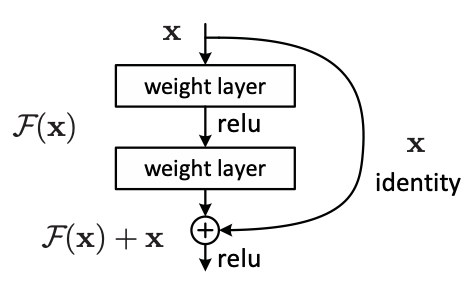
\includegraphics[width=0.5\textwidth]{Figures/resnet/basic.png}
	\caption{Osnovna rezidualna jedinica s preskočnom vezom~\cite{he2016resnet}.}
	\label{fig:resnet-block}
\end{figure}

\subsubsection{Bottleneck blok}

ResNet50 koristi tzv. \textit{bottleneck} blok umjesto osnovnog rezidualnog bloka. Naziv dolazi od karakteristične strukture bloka: konvolucija $1\times1$ prvo smanjuje broj kanala (sužavanje - \textit{bottleneck}), zatim konvolucija $3\times3$ obrađuje smanjenu reprezentaciju, a završna konvolucija $1\times1$ vraća broj kanala na originalnu dimenziju (širenje). Za blok s izlazom od 256 kanala, redoslijed je:

\begin{itemize}
	\item konvolucija $1\times1$, 64 kanala - smanjenje dimenzionalnosti
	\item konvolucija $3\times3$, 64 kanala - prostorna obrada
	\item konvolucija $1\times1$, 256 kanala - vraćanje dimenzionalnosti
\end{itemize}

Ovakva struktura trostruko je računalno učinkovitija od jednog $3\times3$ konvolucijskog sloja s 256 kanala, uz zadržavanje istog receptivnog polja.

\begin{figure}[H]
	\centering
	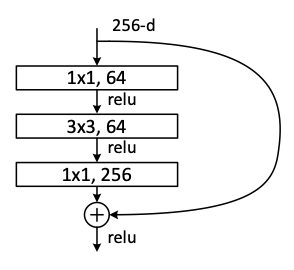
\includegraphics[width=0.4\textwidth]{Figures/resnet/bottleneck.png}
	\caption{ResNet50 bottleneck blok~\cite{he2016resnet}.}
	\label{fig:resnet50block}
\end{figure}

\begin{figure}[H]
	\centering
	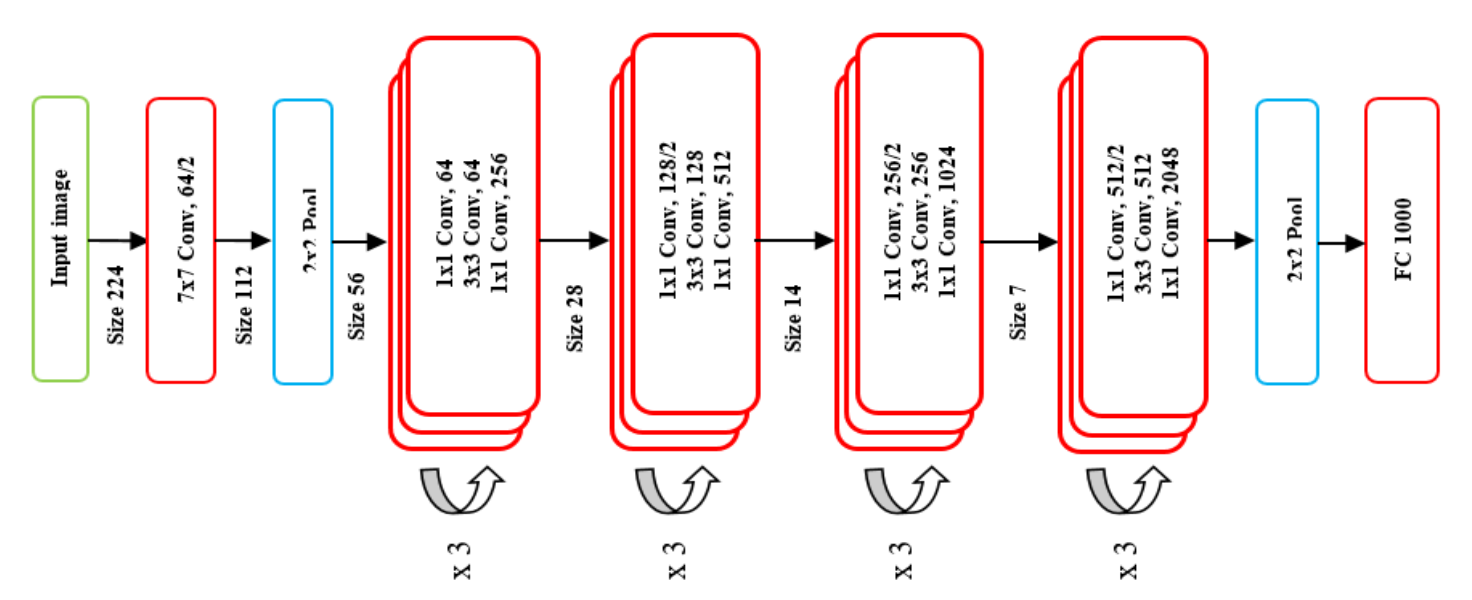
\includegraphics[width=\textwidth]{Figures/resnet/resnet50_architecture.png}
	\caption{Blok dijagram arhitekture ResNet50~\cite{bendjillali2020illumination}.}
	\label{fig:resnet50}
\end{figure}

ResNet50 organiziran je u četiri faze (eng. \textit{stage}), svaka sastavljena od određenog broja bottleneck blokova: 3, 4, 6 i 3 bloka. Prostorne dimenzije mapa značajki smanjuju se između faza, dok broj kanala raste: 256, 512, 1024 i 2048. Izlaz posljednje faze predstavlja mapu značajki dimenzija $\frac{H}{32} \times \frac{W}{32} \times 2048$ za ulaznu sliku dimenzija $H \times W$.

U ovom radu, ova arhitektura koristi se kao okosnica (eng. \textit{backbone}) modela DeepLabV3+, predtrenirana na skupu ImageNet. Hijerarhijske značajke iz više faza kodiraju semantičke informacije na različitim razinama apstrakcije, što je posebno korisno za zadatak semantičke segmentacije gdje je potrebno razumijevanje scene i na globalnoj i na lokalnoj razini.

\subsection{ImageNet predtrening i prijenosno učenje}
\label{sec:transfer_learning}

ImageNet je skup podataka koji sadrži više od 14 milijuna slika raspoređenih u 21\,000 kategorija prema WordNet hijerarhiji~\cite{deng2009imagenet}. U kontekstu dubokog učenja najčešće se koristi podskup od 1000 kategorija i 1.2 milijuna slika poznat kao ILSVRC (eng. \textit{ImageNet Large Scale Visual Recognition Challenge}). Treniranjem na ovom skupu ResNet50 uči bogatu hijerarhiju vizualnih značajki: rani slojevi detektiraju rubove i teksture, srednji slojevi kodiraju dijelove objekata, a duboki slojevi reprezentiraju semantičke koncepte poput kategorija objekata.

Prijenosno učenje (eng. \textit{transfer learning}) označava pristup u kojemu se znanje stečeno rješavanjem jednog zadatka primjenjuje kao polazišna točka za drugi, srodni zadatak~\cite{goodfellow2016deep}. U računalnom vidu standardni tok rada se sastoji od dvije faze: predtreninga okosnice na velikom skupu podataka poput ImageNeta i prilagodbe predtreniranog modela na ciljni zadatak dodavanjem glave specifične za zadatak. Značajke naučene na ImageNetu pokazuju izuzetnu prenosivost na različite zadatke računalnog vida, od detekcije objekata do semantičke segmentacije. Razlog je u tome što su niskorazinske vizualne značajke poput rubova i tekstura, univerzalne i neovisne o specifičnom skupu kategorija~\cite{yosinski2014transferablefeaturesdeepneural}.

U ovom radu, ResNet50 predtreniran na ImageNetu koristi se kao inicijalizacija okosnice modela DeepLabV3+. Ovaj pristup je posebno opravdan s obzirom na relativno mali Cityscapes skup za treniranje (2975 slika), koji sam po sebi ne bi bio dostatan za treniranje dubokih mreža od nule. Predtrening na ImageNetu osigurava kvalitetnu inicijalizaciju težina koja ubrzava konvergenciju i poboljšava konačne performanse segmentacije.



\section{Semantička segmentacija i DeepLabV3+}
\label{sec:segmentacija}

\subsection{Definicija zadatka semantičke segmentacije}

Semantička segmentacija zadatak je računalnog vida koji svakom pikselu ulazne slike dodjeljuje semantičku oznaku iz unaprijed definiranog skupa klasa. Za razliku od klasifikacije slike, koja proizvodi jednu oznaku za cijelu sliku, i detekcije objekata, koja lokalizira objekte graničnim okvirima, semantička segmentacija pruža piksel-precizno razumijevanje scene. Pritom se ne razlikuju pojedinačne instance iste klase. Svi pikseli koji prikazuju automobile dobit će istu oznaku neovisno o njihovom broju.
Standardna metrika za evaluaciju semantičke segmentacije je srednji omjer presjeka i unije (eng. \textit{mean Intersection over Union}, mIoU). Za svaku klasu $i$ računa se IoU kao omjer presjeka i unije predviđene i stvarne maske:

\begin{equation}
	\text{IoU}_i = \frac{\text{TP}_i}{\text{TP}_i + \text{FP}_i + \text{FN}_i}
\end{equation}

gdje su $\text{TP}_i$, $\text{FP}_i$ i $\text{FN}_i$ redom broj točno pozitivnih, lažno pozitivnih i lažno negativnih piksela za klasu $i$. Ukupna metrika mIoU definirana je kao srednja vrijednost IoU-a po svim klasama:

\begin{equation}
	\text{mIoU} = \frac{1}{N_{cl}} \sum_{i=1}^{N_{cl}} \frac{\text{TP}_i}{\text{TP}_i + \text{FP}_i + \text{FN}_i}
\end{equation}

Vrijednost mIoU kreće se između 0 i 1, pri čemu viša vrijednost označava bolju podudarnost predviđenih i stvarnih segmentacijskih maski. Semantička segmentacija nalazi primjenu u brojnim domenama, a posebno je važna u autonomnoj vožnji gdje je potrebno precizno razlikovati voznu površinu, pješake, vozila i infrastrukturu u stvarnom vremenu.

\subsection{Koder-dekoder arhitektura}

Koder-dekoder arhitektura dominantan je pristup u modernoj semantičkoj segmentaciji. Koder je konvolucijska mreža koja postupno smanjuje prostornu rezoluciju ulazne slike ekstrahirajući semantički sve bogatije mape značajki. Dekoder zatim postupno vraća prostornu rezoluciju, dodjeljujući semantičku oznaku svakom pikselu izlazne mape.

Pionirski rad u ovom pristupu bila je potpuno konvolucijska mreža (eng. \textit{Fully Convolutional Network}, FCN) koja je pokazala da konvolucijske mreže za klasifikaciju mogu biti prilagođene za predikciju na razini piksela~\cite{LongSD14}. U-Net je potom uveo preskočne veze (eng. \textit{skip connections}) između odgovarajućih slojeva kodera i dekodera, omogućivši dekoderu pristup niskorazinskim prostornim detaljima koji se gube tijekom koderskog sažimanja~\cite{RonnebergerFB15}. Ove preskočne veze ključne su za preciznu lokalizaciju granica objekata.

\subsection{Dilatacijska (atrous) konvolucija}

Standardna konvolucija s filtrom veličine $k \times k$ može uzeti u obzir samo lokalno susjedstvo piksela. Povećanje receptivnog polja standardnim pristupom zahtijeva ili veće filtre (povećava broj parametara) ili operacije sažimanja (smanjuje prostornu rezoluciju). Dilatacijska konvolucija (eng. \textit{atrous convolution}) elegantno rješava ovaj kompromis uvodeći koeficijent dilatacije $r$ koji definira razmak između aktivnih elemenata filtra~\cite{chen2018deeplabv3plus}:

\begin{equation}
	y[i] = \sum_{k} x[i + r \cdot k]\, w[k]
\end{equation}

gdje $y[i]$ predstavlja izlazni piksel, $x$ je ulazna mapa značajki, $w$ je kernel konvolucije, a $r$ je koeficijent dilatacije. Standardna konvolucija poseban je slučaj za $r = 1$.

\begin{figure}[H]
	\centering
	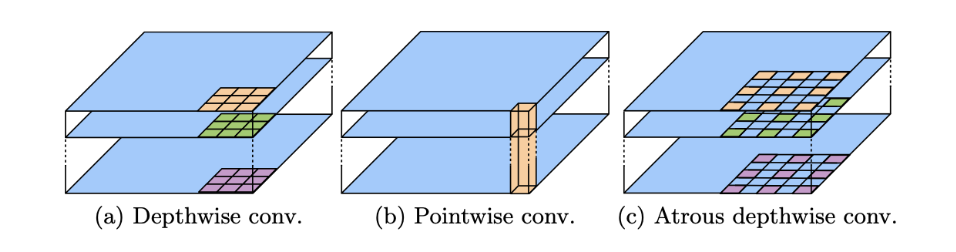
\includegraphics[width=0.75\textwidth]{Figures/deeplab/atrous.png}
	\caption{Vizualni prikaz standardne ($r=1$), točkaste i dilatacijske konvolucije ($r=2$)~\cite{chen2018deeplabv3plus}. Povećanjem koeficijenta dilatacije proširuje se receptivno polje bez povećanja broja parametara.}
	\label{fig:atrous-conv}
\end{figure}

Dilatacijska konvolucija s $r > 1$ proširuje efektivno receptivno polje filtra bez povećanja broja parametara i bez smanjenja prostorne rezolucije. Za segmentaciju je ovo posebno važno jer model može istovremeno analizirati kontekst na više prostornih razina, što je ključno za prepoznavanje objekata različitih veličina.

\subsection{DeepLabV3+ arhitektura}

DeepLabV3+~\cite{chen2018deeplabv3plus} proširenje je modela DeepLabV3 dodatnim dekoderskim modulom koji poboljšava segmentaciju granica objekata. Arhitektura se sastoji od dva glavna dijela: kodera temeljenog na dubokoj konvolucijskoj mreži s ASPP modulom i laganog dekodera koji kombinira visokorazinske i niskorazinske značajke.

\subsubsection{ASPP modul}

Srž kodera je modul Atrous Spatial Pyramid Pooling (ASPP) koji primjenjuje višestruke paralelne dilatacijske konvolucije s različitim koeficijentima dilatacije ($r \in \{6, 12, 18\}$) na istu ulaznu mapu značajki. Svaka grana hvata kontekst na drugoj prostornoj razini, a njihovi izlazi konkateniraju se i kombiniraju konvolucijom $1 \times 1$. Globalno prosječno sažimanje (eng. \textit{global average pooling}) hvata kontekst cijele slike. Na taj način ASPP modul ekstrahira bogatu višerazinsku reprezentaciju koja je robusna na objekte različitih veličina.

\subsubsection{Dekoderski modul}

Za razliku od DeepLabV3 koji izlaz kodera bilinearno interpolira na originalnu rezoluciju, DeepLabV3+ uvodi strukturirani dekoderski modul~\cite{chen2018deeplabv3plus}. Izlaz ASPP modula uvećava se za faktor 4, a zatim se konkatenira s niskorazinskim značajkama iz drugog konvolucijskog bloka kodera koje prolaze kroz konvoluciju $1 \times 1$ za smanjenje broja kanala. Konkatenirana mapa obrađuje se konvolucijama $3 \times 3$ i konačno interpolira na originalnu rezoluciju slike.

\begin{figure}[H]
	\centering
	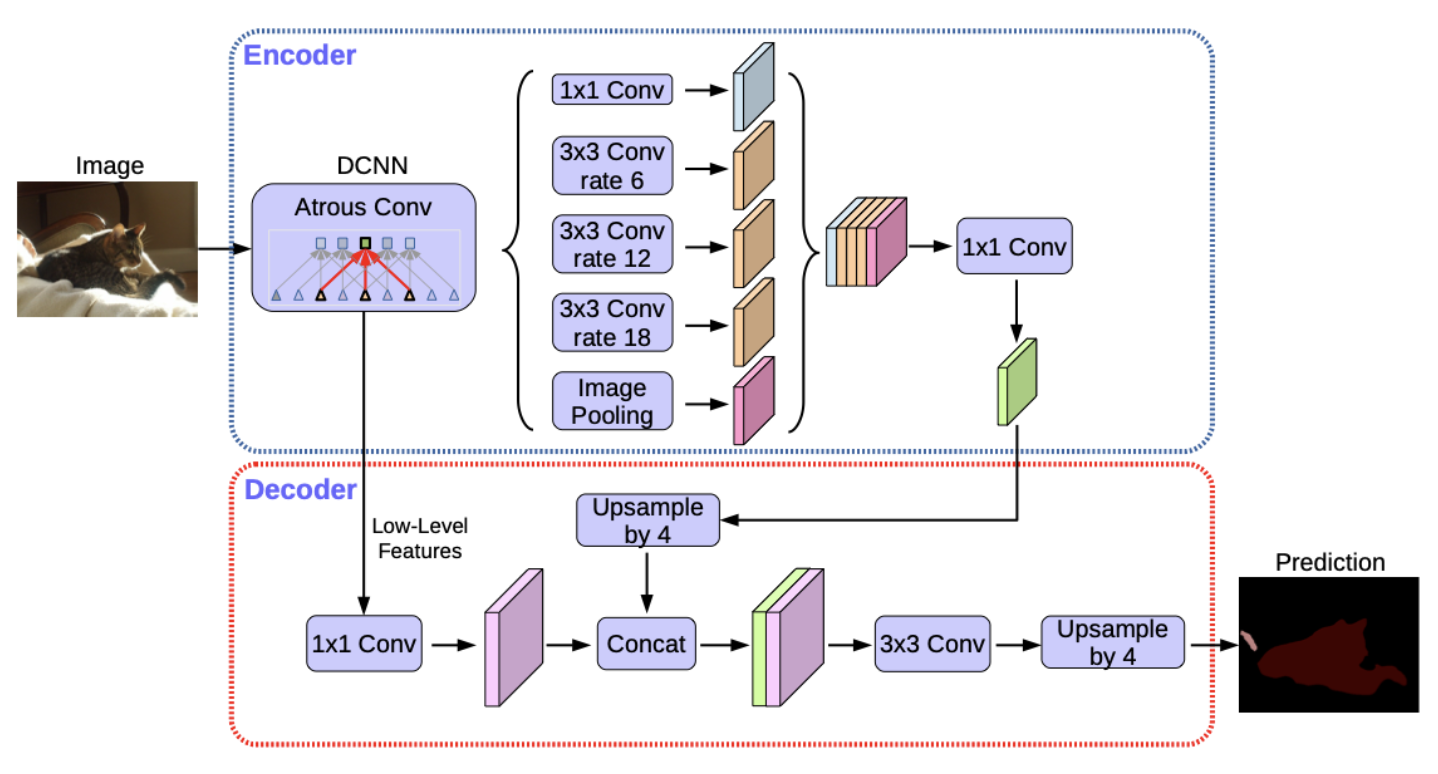
\includegraphics[width=\textwidth]{Figures/deeplab/architecture.png}
	\caption{Arhitektura koder-dekoder modela DeepLabV3+~\cite{chen2018deeplabv3plus}.}
	\label{fig:deeplabv3plus}
\end{figure}


\section{Samonadzirano učenje}
\label{sec:ssl}

\subsection{Motivacija i definicija samonadziranog učenja}

Nadzirano učenje (eng. \textit{supervised learning}) postiglo je izvanredne rezultate u računalnom vidu, no njegova primjena pretpostavlja dostupnost velikih količina ručno označenih podataka. Prikupljanje i označavanje podataka skupo je i vremenski zahtjevno jer anotacija jedne Cityscapes slike na razini piksela zahtijeva u prosjeku 1.5 sat rada~\cite{cordts2016cityscapes}. S druge strane, neoznačenih vizualnih podataka ima u izobilju: videozapisi s prometnih kamera, snimke autonomnih vozila i internetski sadržaj predstavljaju gotovo neiscrpan izvor sirovih podataka.

Samonadzirano učenje (eng. \textit{self-supervised learning}, SSL) pristup je koji rješava ovaj jaz iskorištavanjem strukture samih podataka kao nadzornog signala, bez potrebe za ručnim anotacijama~\cite{goodfellow2016deep}. Model se trenira na tzv. \textit{pretext} zadacima koji se automatski generiraju iz neoznačenih podataka, a čije rješavanje zahtijeva razumijevanje semantičke strukture ulaza.

Primjeri klasičnih pretext zadataka uključuju:
\begin{itemize}
	\item \textbf{Predviđanje rotacije} - modelu se prikazuje slika rotirana za $0^{\circ}$, $90^{\circ}$, $180^{\circ}$ ili $270^{\circ}$ i od njega se traži klasifikacija kuta rotacije~\cite{goodfellow2016deep}
	\item \textbf{Jigsaw puzzle} - slika se izrezuje na segmente koji se nasumično permutiraju, a model uči rekonstruirati originalnu permutaciju
	\item \textbf{Kolorizacija} - modelu se prikazuje slika u sivim tonovima i od njega se traži predikcija boje svakog piksela
\end{itemize}

Pretext zadaci su pomoćni mehanizam. Cilj nije naučiti sam zadatak, već prisiliti model da razvije korisne vizualne reprezentacije koje se mogu prenijeti na zadatke poput klasifikacije, detekcije ili segmentacije. U modernom SSL-u dominiraju metode kontrastivnog učenja koje ne zahtijevaju eksplicitni pretext zadatak, već direktno optimiziraju strukturu prostora reprezentacija, što je opisano u sljedećem odjeljku.

\subsection{Kontrastivno učenje}

Kontrastivno učenje (eng. \textit{contrastive learning}) pristup je samonadziranog učenja koji uči reprezentacije izravnom optimizacijom strukture prostora značajki, bez eksplicitnog pretext zadatka. Temeljna ideja je jednostavna: reprezentacije semantički sličnih uzoraka trebaju biti blizu u prostoru značajki, dok reprezentacije semantički različitih uzoraka trebaju biti daleko~\cite{chen2020simclr, he2020moco}.

Za svaki ulazni primjer $x$ generiraju se dva pogleda $x^+_1$ i $x^+_2$ primjenom nasumičnih augmentacija. Ova dva pogleda čine \textit{pozitivni par}. Pretpostavlja se da, budući da potječu od istog primjera, dijele semantički sadržaj. Svi ostali primjeri u skupu za treniranje tretiraju se kao \textit{negativni primjeri}. Model uči kodirati pozitivne parove u slične vektore, a negativne u različite.

Standardna funkcija gubitka za kontrastivno učenje je InfoNCE (eng. \textit{Information Noise-Contrastive Estimation})~\cite{he2020moco}:

\begin{equation}
	\mathcal{L}_{\text{InfoNCE}} = -\log \frac{\exp(\mathbf{q} \cdot \mathbf{k}^+ / \tau)}{\exp(\mathbf{q} \cdot \mathbf{k}^+ / \tau) + \sum_{i=1}^{N} \exp(\mathbf{q} \cdot \mathbf{k}^-_i / \tau)}
\end{equation}

gdje je $\mathbf{q}$ reprezentacija upita (eng. \textit{query}), $\mathbf{k}^+$ reprezentacija pozitivnog para, $\mathbf{k}^-_i$ reprezentacije negativnih primjera, a $\tau$ temperatura koja kontrolira oštrost distribucije. Minimizacijom ovog gubitka model uči razlikovati pozitivni par od negativnih primjera, zadatak analogan $(N+1)$-razrednoj klasifikaciji.

Broj negativnih primjera $N$ ključan je hiperparametar: veći broj negativnih primjera daje bolji signal za učenje, ali zahtijeva veće memorijske i računalne resurse. Ovo ograničenje motiviralo je razvoj arhitektura poput MoCo koje rješavaju problem velikog broja negativnih primjera bez potrebe za velikim skupnim veličinama.

\subsection{MoCo v2}
\label{sec:mocov2}

Momentum Contrast (MoCo)~\cite{he2020moco} i njegova poboljšana inačica MoCo v2~\cite{chen2020improvedbaselinesmomentumcontrastive} uveli su arhitekturu s dva kodera i pohranom negativnih primjera koja omogućuje učinkovito kontrastivno učenje na jednom grafičkom procesoru s umjerenim skupnim veličinama.

\begin{figure}[H]
	\centering
	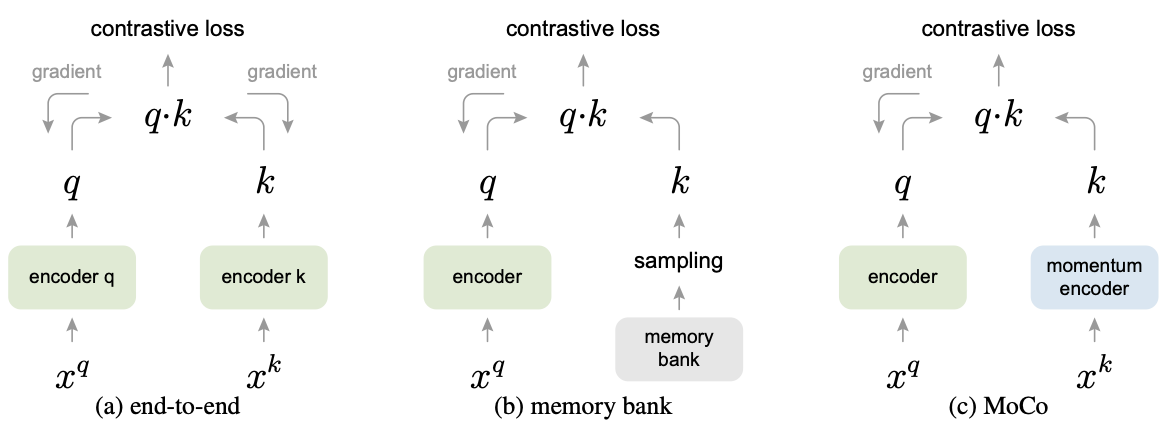
\includegraphics[width=\textwidth]{Figures/moco/moco_comparison.png}
	\caption{Tri pristupa kontrastivnom učenju: end-to-end, memory bank 
		i Momentum Contrast (MoCo). MoCo koristi momentum koder i 
		pohranu ključeva koja odspaja broj negativnih primjera od 
		skupne veličine~\cite{he2020moco}.}
	\label{fig:moco-comparison}
\end{figure}

\subsubsection{Arhitektura s dva kodera}

MoCo v2 koristi dva kodera: koder upita $f_q$ i koder ključa $f_k$. Koder upita trenira se gradijentnim spustom, dok se koder ključa ažurira sporim eksponencijalnim usrednjavanjem (eng. \textit{momentum update}) parametara kodera upita:

\begin{equation}
	\theta_k \leftarrow m \cdot \theta_k + (1 - m) \cdot \theta_q
\end{equation}

gdje je $m \in [0, 1)$ koeficijent momenta, tipično $m = 0.99$. Ovakvo ažuriranje osigurava da koder ključa evoluira sporije od kodera upita, čime se postiže konzistentnost reprezentacija pohrane negativnih primjera.

Oba kodera sastoje se od okosnice ResNet50 i dvoslojne MLP projekcijske glave koja preslikava značajke u $\ell_2$-normalizirani prostor dimenzije 128. $\ell_2$ normalizacija osigurava da se sličnost mjeri kosinusnim produktom, a ne euklidskom udaljenošću.

\subsubsection{Pohrana negativnih primjera}

Ključna inovacija MoCo arhitekture je pohrana negativnih primjera (eng. \textit{queue}) koja odspaja broj negativnih primjera od skupne veličine. Pohrana sadrži $M$ najrecentnijih reprezentacija ključeva (tipično $M = 65536$), koje se ažuriraju kliznim prozorom: na svakom koraku treniranja nove reprezentacije dodaju se na kraj pohrane, a najstarije se uklanjaju s početka.

Ovaj pristup omogućuje veliki broj negativnih primjera (što je važno za kvalitetu učenja) bez potrebe za velikim skupnim veličinama koje bi zahtijevale višestruke grafičke procesore~\cite{he2020moco}.

\subsubsection{MoCo v2 poboljšanja}

MoCo v2~\cite{chen2020improvedbaselinesmomentumcontrastive} donosi dva ključna poboljšanja u odnosu na originalnu MoCo arhitekturu: zamjenu linearne projekcijske glave dvoslojnom MLP glavom s ReLU aktivacijom, te jači augmentacijski skup koji uključuje Gaussovo zamagljivanje. Oba poboljšanja preuzeta su iz SimCLR~\cite{chen2020simclr} i značajno poboljšavaju kvalitetu naučenih reprezentacija.

\subsubsection{Relevantnost za ovaj rad}

MoCo v2 odabran je kao metoda samonadziranog predtreninga u ovom radu zbog nekoliko prednosti. Kao prvo, pohrana negativnih primjera omogućuje učinkovito kontrastivno učenje na jednom grafičkom procesoru (NVIDIA A100) s umjerenom skupnom veličinom od 256, bez potrebe za sinkronizacijom gradijenata između više procesora. Kao drugo, MoCo v2 je dobro proučena i reproducibilna metoda s jasno definiranim hiperparametrima. Kao treće, arhitektura s dva kodera prirodno se prilagođava temporalnoj modifikaciji opisanoj u nastavku.

\subsection{Temporal kontrastivno učenje}

Temporal kontrastivno učenje pristup je koji kao pozitivne parove koristi uzorke koji su vremenski blizu u video sekvenci, umjesto augmentacija iste slike~\cite{cvrl2021}. Temeljna pretpostavka je da susjedni okviri video sekvence prikazuju semantički sličan sadržaj: ista scena, isti objekti, male promjene zbog kretanja kamere ili objekata. Ova temporalna konzistencija može poslužiti kao prirodni nadzorni signal za učenje korisnih vizualnih reprezentacija.

Pristup je posebno motiviran za domenu prometnih scena: Cityscapes-Sequence sadrži kontinuirane videozapise snimljene iz automobila u kojima susjedni okviri prikazuju gotovo identičnu scenu. Temporalni signal tjera model da nauči reprezentacije koje su robusne na manje prostorne i fotometrijske varijacije između okvira. Takva vrsta invarijantnosti korisna je za detekciju anomalija, gdje model treba prepoznati nepoznate objekte neovisno o točnoj perspektivi ili osvjetljenju.

Srodni radovi koji su istraživali temporal kontrastivno učenje uključuju CVRL~\cite{cvrl2021} koji uvodi kontrastivno učenje na video sekvencama koristeći augmentacije prostornog i temporalnog susjedstva, te VideoMoCo~\cite{pan2021videomoco} koji proširuje MoCo arhitekturu na video domenu uvođenjem temporalno svjesne pohrane negativnih primjera.

U ovom radu predlaže se jednostavna, ali učinkovita modifikacija standardnog MoCo v2 algoritma: pozitivni par definira se kao dva okvira iz iste video sekvence unutar maksimalnog vremenskog pomaka, umjesto dvaju pogleda iste slike. Detalji implementacije opisani su u poglavlju~\ref{sec:ssl_predtrening}.




\section{Detekcija anomalija u semantičkoj segmentaciji}
\label{sec:anomaly_detection}

\subsection{Izvandistribucijska detekcija}

Modeli dubokog učenja trenirani na zatvorenom skupu klasa pretpostavljaju da će ulazni podatci tijekom zaključivanja (eng. \textit{inference}) dolaziti iz iste distribucije kao i podatci za treniranje. U stvarnim uvjetima autonomne vožnje ova pretpostavka često nije zadovoljena. Na cesti se mogu pojaviti objekti koji se ne nalaze ni u jednoj od poznatih klasa, poput divljih životinja, izgubljenog tereta ili neočekivanih prepreka. Takvi primjeri nazivaju se izvandistribucijskim uzorcima (eng. \textit{out-of-distribution}, OOD).

Formalno, neka je $\mathcal{D}_{in}$ distribucija podataka za treniranje s poznatim skupom klasa $\mathcal{Y} = \{1, \ldots, K\}$. Model $f_\theta$ treniran na $\mathcal{D}_{in}$ uči preslikavanje $f_\theta: \mathcal{X} \rightarrow \mathcal{Y}$. OOD detekcija zadatak je prepoznavanja ulaznih primjera koji ne potječu iz $\mathcal{D}_{in}$, tj. primjera čija prava klasa nije sadržana u $\mathcal{Y}$~\cite{chan2021segmentmeifyoucanbenchmarkanomalysegmentation}. U kontekstu ovog rada, $\mathcal{D}_{in}$ je skup Cityscapes s 19 klasa prometnih scena, a OOD primjeri su svi objekti koji se ne mogu svrstati ni u jednu od tih klasa.

Ključan uvid koji motivira post-hoc pristupe detekciji anomalija leži u ponašanju modela semantičke segmentacije na OOD uzorcima: model koji nije vidio određeni objekt tijekom treniranja tipično daje nesigurnu i raspršenu distribuciju vjerojatnosti po klasama umjesto pouzdane predikcije jedne klase~\cite{hendrycks2017baseline}. Ta se nesigurnost može iskoristiti kao signal za detekciju anomalija bez ikakvih izmjena u procesu treniranja.

\subsection{Detekcija na razini piksela u odnosu na razinu slike}

OOD detekcija može se provoditi na dvjema prostornim razinama: razini slike i razini piksela.

Detekcija na razini slike (eng. \textit{image-level}) dodjeljuje jednu binarnu odluku cijeloj slici. Slika je ili normalna ili anomalna. Ovaj pristup je računalno jednostavan i prikladan za scenarije gdje je dovoljna gruba lokalizacija. Međutim, u prometnim scenama anomalija tipično zauzima samo mali dio slike (životinja na cesti, prepreka u jednoj prometnoj traci), dok ostatak scene ostaje posve normalan. Dodjela jedne oznake cijeloj slici gubi tu prostornu informaciju i nije operativno korisna za sustave autonomne vožnje koji trebaju znati točnu lokaciju opasnosti.

Detekcija na razini piksela (eng. \textit{pixel-level}) svakom pikselu ulazne slike neovisno dodjeljuje anomalni rezultat, čime se dobiva prostorno precizna karta anomalija. Ovaj pristup odgovara paradigmi semantičke segmentacije. Isti model koji klasificira svaki piksel u poznatu klasu može istovremeno označiti piksele koji ne odgovaraju ni jednoj poznatoj klasi~\cite{chan2021segmentmeifyoucanbenchmarkanomalysegmentation}.

U ovom radu koristi se isključivo detekcija na razini piksela, budući da benchmark SegmentMeIfYouCan mjeri pikselnu preciznost detekcije te da sustavi autonomne vožnje zahtijevaju prostornu lokalizaciju anomalija.

\subsection{Funkcije za ocjenu anomalija}

Funkcije za ocjenu anomalija (eng. \textit{anomaly scoring functions}) transformiraju logite segmentacijskog modela u skalarne vrijednosti koje odražavaju stupanj anomalnosti pojedinog piksela. Sve tri korištene funkcije su tzv.\ post-hoc metode, primjenjuju se na već trenirani model bez ikakvih izmjena u procesu treniranja.

Neka je $\mathbf{z} = (z_1, \ldots, z_K) \in \mathbb{R}^K$ vektor logita za jedan piksel, gdje je $K = 19$ broj Cityscapes klasa. Softmax transformacija daje distribuciju vjerojatnosti:

\begin{equation}
	p_k = \frac{e^{z_k}}{\sum_{j=1}^{K} e^{z_j}}, \quad k = 1, \ldots, K
\end{equation}

\subsubsection{Maximum Softmax Probability (MSP)}

MSP metodu predložili su Hendrycks i Gimpel~\cite{hendrycks2017baseline} kao prvu sustavnu osnovnu metodu (eng. \textit{baseline}) za OOD detekciju. Anomalni rezultat definiran je kao komplement maksimalne softmax vjerojatnosti:

\begin{equation}
	s_{\text{MSP}}(\mathbf{z}) = 1 - \max_{k} \, p_k
\end{equation}

Intuicija je jednostavna: model koji je siguran u svoju predikciju daje visoku vjerojatnost jednoj klasi, dok nesiguran model suočen s OOD uzorkom raspoređuje vjerojatnost ravnomjernije. Visok MSP anomalni rezultat odgovara niskoj maksimalnoj vjerojatnosti, tj. visokoj nesigurnosti modela.

\subsubsection{Maximum Logit Score}

Hendrycks i suradnici~\cite{hendrycks2019scaling} pokazali su da rad izravno s logitima, bez softmax normalizacije, daje bolje rezultate. Anomalni rezultat definiran je kao negativ maksimalnog logita:

\begin{equation}
	s_{\text{MaxLogit}}(\mathbf{z}) = -\max_{k} \, z_k
\end{equation}

Prednost nad MSP-om leži u tome što softmax transformacija komprimira logite u interval $[0, 1]$ i pritom gubi informaciju o apsolutnoj veličini logita. Modeli trenirani na unutardistribucijskim podatcima produciraju visoke logite za poznate klase, dok za OOD uzorke svi logiti ostaju relativno niski.

\subsubsection{Energy Score}

Liu i suradnici~\cite{liu2020energybasedoutdistributiondetection} uveli su energetski rezultat motiviran teorijom energetskih modela (eng. \textit{energy-based models}). Za vektor logita $\mathbf{z}$, energija je definirana kao:

\begin{equation}
	E(\mathbf{z}) = -\log \sum_{k=1}^{K} e^{z_k}
\end{equation}

Anomalni rezultat je negativna energija:

\begin{equation}
	s_{\text{Energy}}(\mathbf{z}) = -E(\mathbf{z}) = \log \sum_{k=1}^{K} e^{z_k}
\end{equation}

Viši energetski rezultat odgovara većoj vjerojatnosti da je piksel anomalan. Teorijska motivacija: za unutardistribucijske uzorke barem jedan logit je visok, što čini sumu eksponenata velikom i energiju niskom. Za OOD uzorke svi su logiti umjereni, suma eksponenata je manja, a energija viša.

\subsection{Pregled relevantnih metoda}

Posljednjih godina razvijen je niz specijaliziranih metoda za detekciju anomalija u semantičkoj segmentaciji koje značajno nadmašuju post-hoc pristupe opisane u prethodnom odjeljku.

\textbf{Outlier Exposure} tehnika je u kojoj se model trenira uz dodatni skup podataka koji sadrži uzorke izvan distribucije treniranja~\cite{chan2021segmentmeifyoucanbenchmarkanomalysegmentation}. Model eksplicitno uči razlikovati unutardistribucijske od OOD uzoraka, što tipično daje znatno bolje rezultate. Međutim, ovaj pristup zahtijeva pažljiv odabir OOD podataka za treniranje i pretpostavlja određeno predznanje o vrsti anomalija koje se mogu pojaviti.

\textbf{PEBAL}~\cite{tian2022pebal} kombinira energetski trening s pikselnom Bayesovom procjenom izglednosti. Model se dodatno dotrenira uz energetski gubitak koji eksplicitno povećava energiju OOD uzoraka i smanjuje energiju unutardistribucijskih uzoraka, koristeći uzorke iz skupa COCO kao zamjenske OOD podatke.

\textbf{Mask2Anomaly}~\cite{rai2023mask2anomaly} temelji se na arhitekturi Mask2Former za panoptičku segmentaciju. Anomalije se detektiraju kao regije koje ne odgovaraju ni jednoj naučenoj masci objekta, što omogućuje prirodnu integraciju detekcije anomalija u segmentacijski postupak bez posebnih OOD gubitaka.

\textbf{RbA}~\cite{nayal2023rba} (eng. \textit{Residual by Aggregation}) agregira rezidualne značajke iz više razina kodera kako bi dobio robustan anomalni rezultat, pokazujući da su niskorazinske značajke posebno informativne za detekciju anomalija.

U ovom radu namjerno je odabran post-hoc pristup bez outlier exposurea iz nekoliko razloga. Kao prvo, cilj rada nije razvoj nove metode detekcije anomalija, već istraživanje utjecaja samonadziranog predtreninga na kvalitetu naučenih reprezentacija. Kao drugo, post-hoc pristup omogućuje poštenu usporedbu triju modela (osnovni model, MoCo standard, MoCo temporal) budući da se jedina razlika između njih nalazi u inicijalizaciji okosnice, a ne u metodi detekcije. Kao treće, post-hoc metode ne zahtijevaju OOD podatke za treniranje, što ih čini primjenjivima u scenarijima gdje vrsta budućih anomalija nije poznata unaprijed.




%-------------------------------------------------------------------------------
\chapter{Skup podataka}
\label{pog:skup_podataka}



\section{Cityscapes}
\label{sec:cityscapes}

\subsection{Pregled skupa podataka}

Skup podataka (eng. \textit{dataset}) Cityscapes sadrži podatke urbanih scena koje prikazuju situacije na ulici tijekom vožnje. Cilj skupa podataka je izvlačenje semantičkog razumijevanja urbanih prometnih scena. Anotacije pokrivaju gustu semantičku segmentaciju i segmentaciju instanci automobila te ljudi. Podatci su snimani u 50 gradova tijekom nekoliko mjeseci kroz različita godišnja doba po dnevnom svjetlu uz dobre do srednje vremenske uvjete. Scene prikazuju velik broj dinamičkih objekata s varijabilnim pozadinama i kompozicijama scena. Za snimanje je korištena video kamera koja snima videozapise rezolucije 2048$\times$1024 piksela. Skup podataka objavili su istraživači iz Daimler AG-a u suradnji s Max Planck institutom i Tehničkim sveučilištem u Darmstadtu 2016. godine \cite{cordts2016cityscapes}. Skup podataka sadrži metapodatke poput GPS lokacije i temperature okoliša, koji nisu korišteni u ovom radu.

\subsection{Anotacije i klase}

Cityscapes sadrži 5000 fino označenih primjera i 20000 grubo označenih primjera. U implementaciji su korišteni isključivo fino označeni primjeri.

\begin{figure}[h]
	\centering
	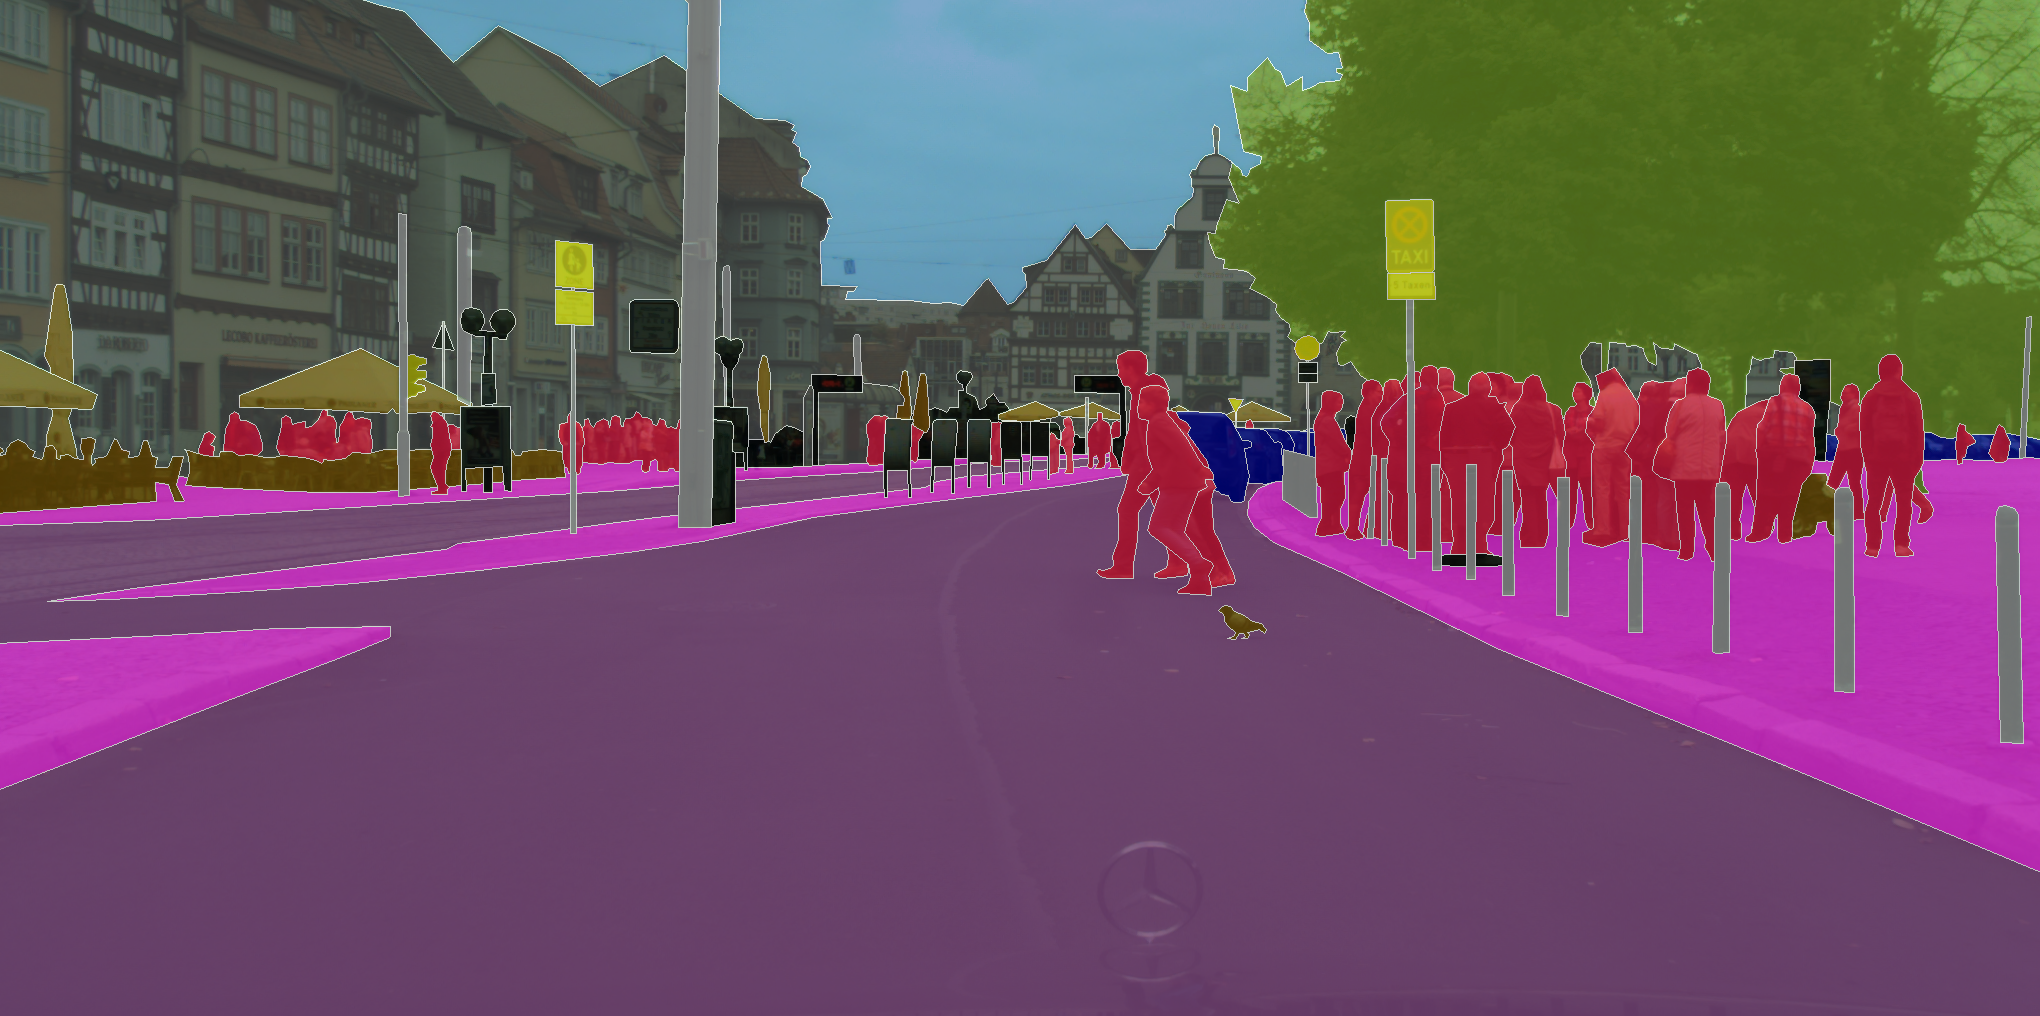
\includegraphics[width=0.48\textwidth]{Figures/cityscapes/cityscapes_fine.png}
	\hfill
	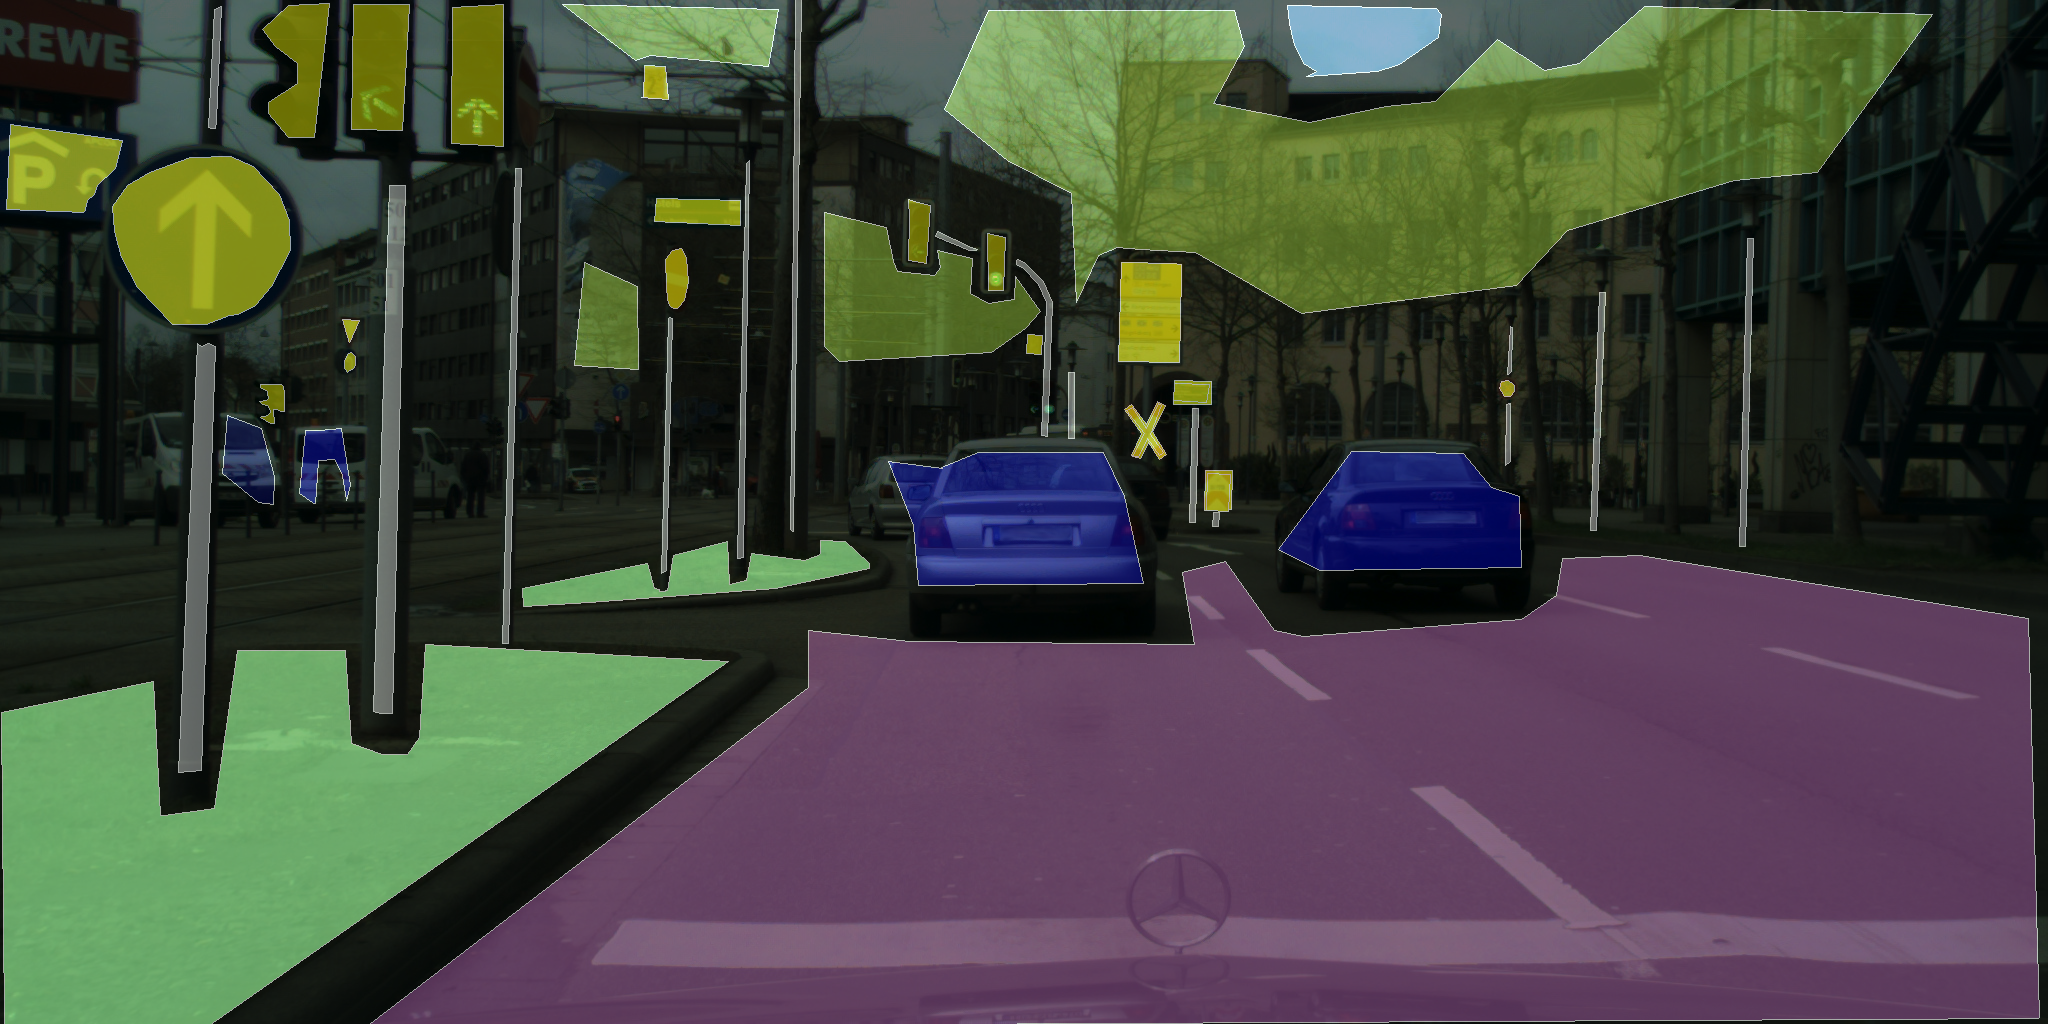
\includegraphics[width=0.48\textwidth]{Figures/cityscapes/cityscapes_coarse.png}
	\caption{Primjer fino označene (lijevo) i grubo označene (desno) anotacije iz Cityscapes skupa podataka.}
	\label{fig:cityscapes-annotations}
\end{figure}

Skup podataka definira ukupno 30 klasa raspoređenih u 8 kategorija, od kojih se 19 koristi u standardnom evaluacijskom protokolu. Klase označene s $^{+}$ isključene su iz evaluacije zbog rijetke pojavnosti ili nejasnih granica, dok se klase označene s $^{*}$ evaluiraju i na razini instanci.

\begin{table}[h]
	\centering
	\caption{Cityscapes ontologija klasa. Klase označene s $^{*}$ evaluiraju se na razini instanci, klase označene s $^{+}$ nisu uključene u standardni 19-klasni eval protokol.}
	\label{tab:cityscapes-classes}
	\begin{tabular}{|l|l|}
		\hline
		\textbf{Kategorija} & \textbf{Klase} \\
		\hline
		flat         & road, sidewalk, parking$^{+}$, rail track$^{+}$ \\
		human        & person$^{*}$, rider$^{*}$ \\
		vehicle      & car$^{*}$, truck$^{*}$, bus$^{*}$, on rails$^{*}$, motorcycle$^{*}$, bicycle$^{*}$, caravan$^{*+}$, trailer$^{*+}$ \\
		construction & building, wall, fence, guard rail$^{+}$, bridge$^{+}$, tunnel$^{+}$ \\
		object       & pole, pole group$^{+}$, traffic sign, traffic light \\
		nature       & vegetation, terrain \\
		sky          & sky \\
		void         & ground$^{+}$, dynamic$^{+}$, static$^{+}$ \\
		\hline
	\end{tabular}
\end{table}

\subsection{Podjela na trening, validaciju i test}

Fino označeni skup podataka podijeljen je na tri dijela: 2975 slika za treniranje, 500 slika za validaciju i 1525 slika za testiranje. Skup za testiranje nije korišten u ovom radu jer su anotacije segmentacijskih maski privatne, odnosno dostupne isključivo putem službenih evaluacijskih poslužitelja. Evaluacija semantičke segmentacije provedena je na validacijskom skupu od 500 slika, pri čemu se kao standardna metrika koristi srednji omjer presjeka i unije (eng. \textit{mean Intersection over Union}, mIoU).

\subsection{Cityscapes-Sequence}

Uz standardni segmentacijski skup postoji Cityscapes-Sequence. To je proširenje koje za svaku sliku iz skupa za treniranje uključuje 30 uzastopnih okvira snimljenih neposredno prije i nakon nje. Ukupno 89\,750 slika bez semantičkih oznaka snimljenih brzinom 17 FPS (eng. \textit{frames per second}), što odgovara otprilike 1.8 sekundi po isječku.

\begin{figure}[h]
	\centering
	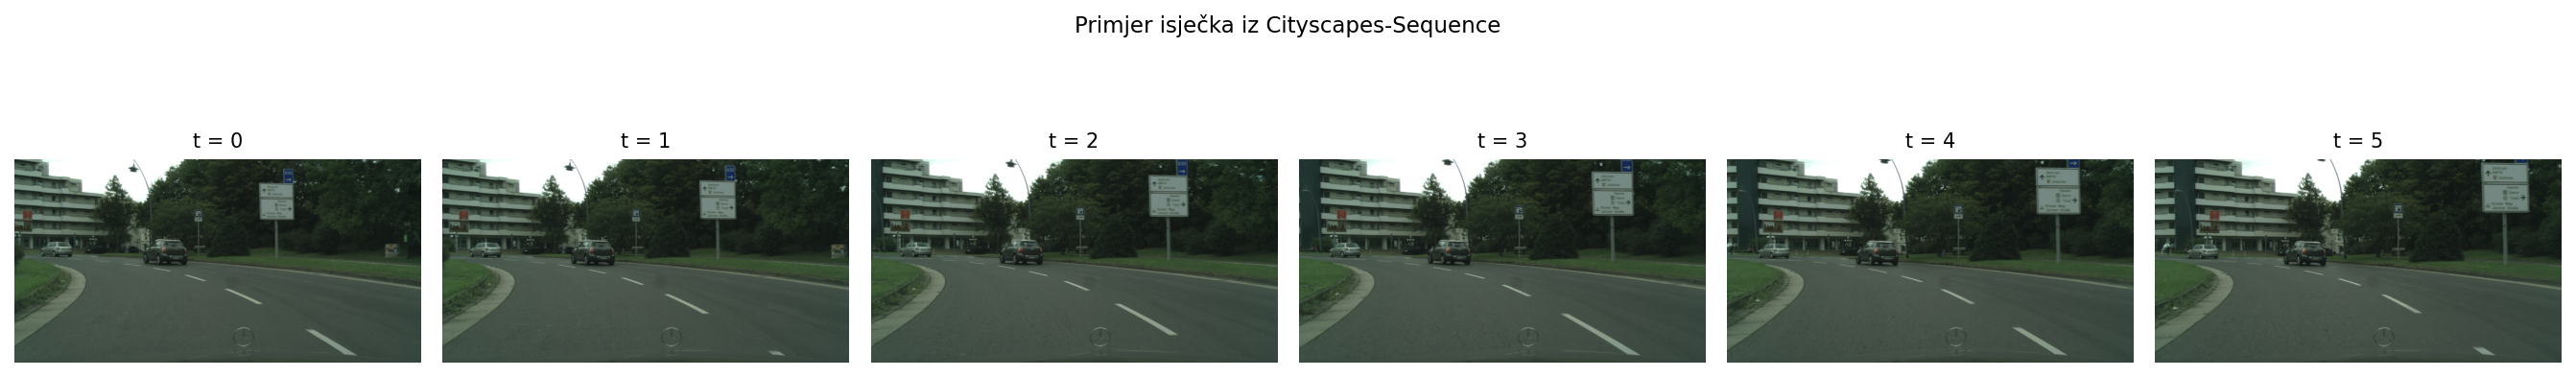
\includegraphics[width=\textwidth]{Figures/cityscapes/cityscapes_sequence.png}
	\caption{Primjer isječka iz Cityscapes-Sequence skupa podataka. Prikazano je nekoliko uzastopnih okvira iz iste sekvence, bez semantičkih anotacija.}
	\label{fig:cityscapes-sequence}
\end{figure}

U ovom radu Cityscapes-Sequence koristi se isključivo u fazi samonadziranog predtreninga. Budući da slike nemaju anotacije, ne mogu se koristiti za nadzirano učenje, ali bogata temporalna struktura čini ih pogodnim za kontrastivno učenje. Svaki okvir tretira se kao sidro (eng. \textit{anchor}), a kao pozitivni par bira se nasumični okvir iz istog isječka unutar maksimalnog vremenskog pomaka od 15 koraka. Na taj način model uči reprezentacije konzistentne kroz vrijeme, što je ključna motivacija za uvođenje temporalne komponente MoCo v2 algoritma opisane u poglavlju~\ref{sec:temporal-moco}.

Radi ubrzanja učitavanja podataka, sve slike su prethodno smanjene s izvorne rezolucije 2048$\times$1024 na 512$\times$256 piksela i spremljene u JPEG formatu. Ova prilagodba smanjuje I/O opterećenje bez značajnog utjecaja na kvalitetu naučenih reprezentacija, budući da se tijekom treninga iz svake slike izrezuju nasumični isječci veličine 224$\times$224 piksela.



\section{SegmentMeIfYouCan}
\label{sec:smiyc}

SegmentMeIfYouCan (SMIYC) benchmark~\cite{chan2021segmentmeifyoucanbenchmarkanomalysegmentation} osmišljen je za evaluaciju metoda detekcije anomalija u prometnim scenama na razini piksela. Modeli semantičke segmentacije trenirani na zatvorenim skupovima klasa, poput Cityscapes skupa s 19 klasa, nisu sposobni prepoznati objekte koji se ne pojavljuju u skupu za treniranje. SMIYC mjeri koliko uspješno model detektira takve nepoznate objekte, pri čemu modeli ulaze isključivo s pikselima višeg anomalnog rezultata za objekte izvan poznatih klasa.

Benchmark se sastoji od dvaju zasebnih skupova podataka koji pokrivaju dvije različite vrste anomalija: RoadAnomaly21 i RoadObstacle21.

\subsection{RoadAnomaly21}

RoadAnomaly21 sadrži slike prometnih scena s raznolikim anomalijama prikupljenim s interneta, npr. životinje, neobična vozila i nasumični objekti koji se ne pojavljuju u skupu za treniranje. Scene su vizualno raznolike i ne potječu nužno iz perspektive vozača automobila. Skup se sastoji od 100 test slika sa skrivenim anotacijama i 10 validacijskih slika s javno dostupnim anotacijama. Sve slike su rezolucije 1280$\times$720 piksela.

\begin{figure}[h]
	\centering
	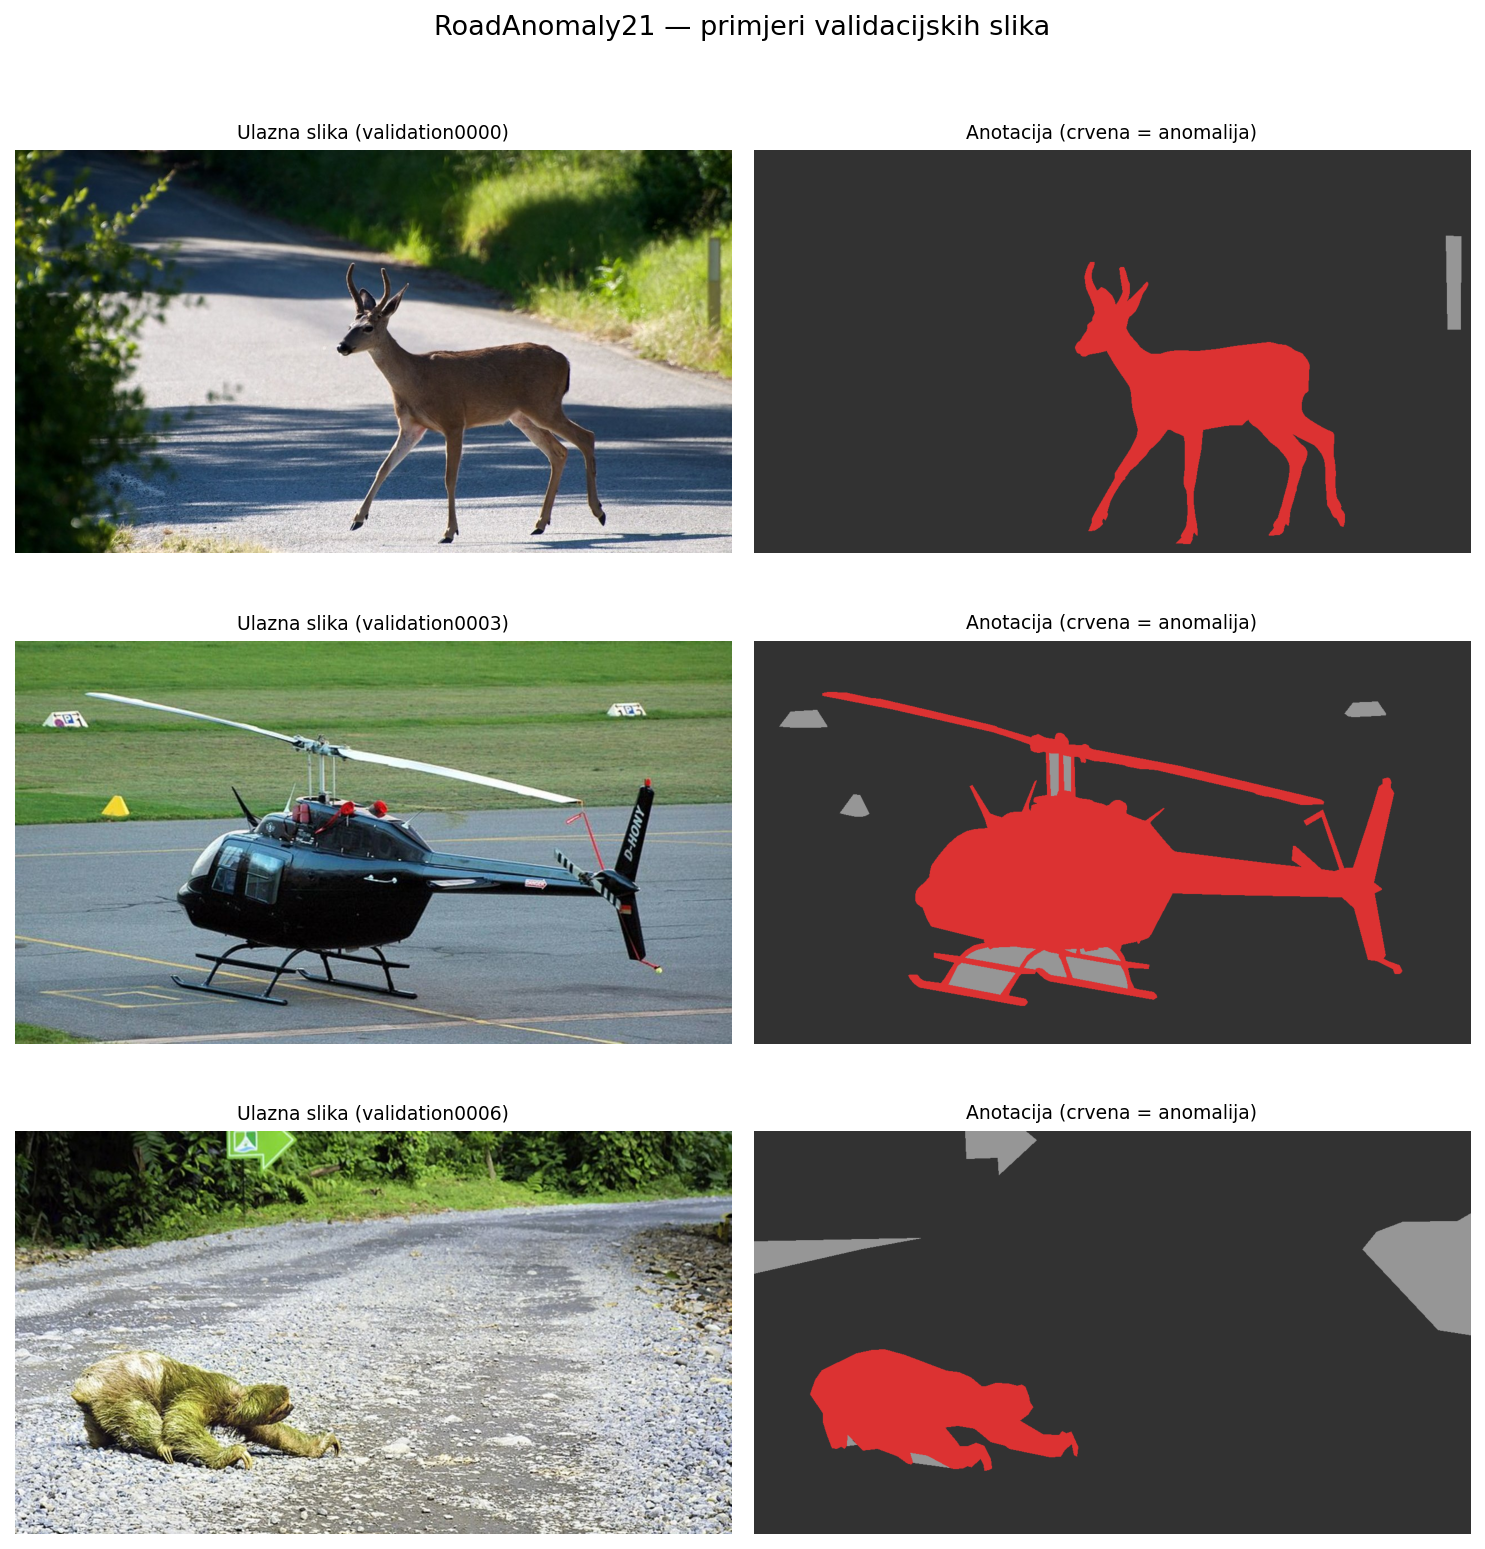
\includegraphics[width=\textwidth]{Figures/smiyc/smiyc_anomaly_examples.png}
	\caption{Primjeri iz RoadAnomaly21 skupa podataka s pripadajućim anotacijama. Crvena boja označava anomalne piksele.}
	\label{fig:smiyc-anomaly}
\end{figure}

\subsection{RoadObstacle21}

RoadObstacle21 sadrži slike stvarnih objekata postavljenih na cestu i snimljenih u kontroliranim uvjetima. Prepreke uključuju kutije, kanistre, životinje i igračke na različitim vrstama podloge: asfaltu, šljunku, pločniku i autocesti. Skup sadrži 327 test slika sa skrivenim anotacijama i 30 validacijskih slika s javnim anotacijama. Rezolucija slika je 1920$\times$1080 piksela.

\begin{figure}[H]
	\centering
	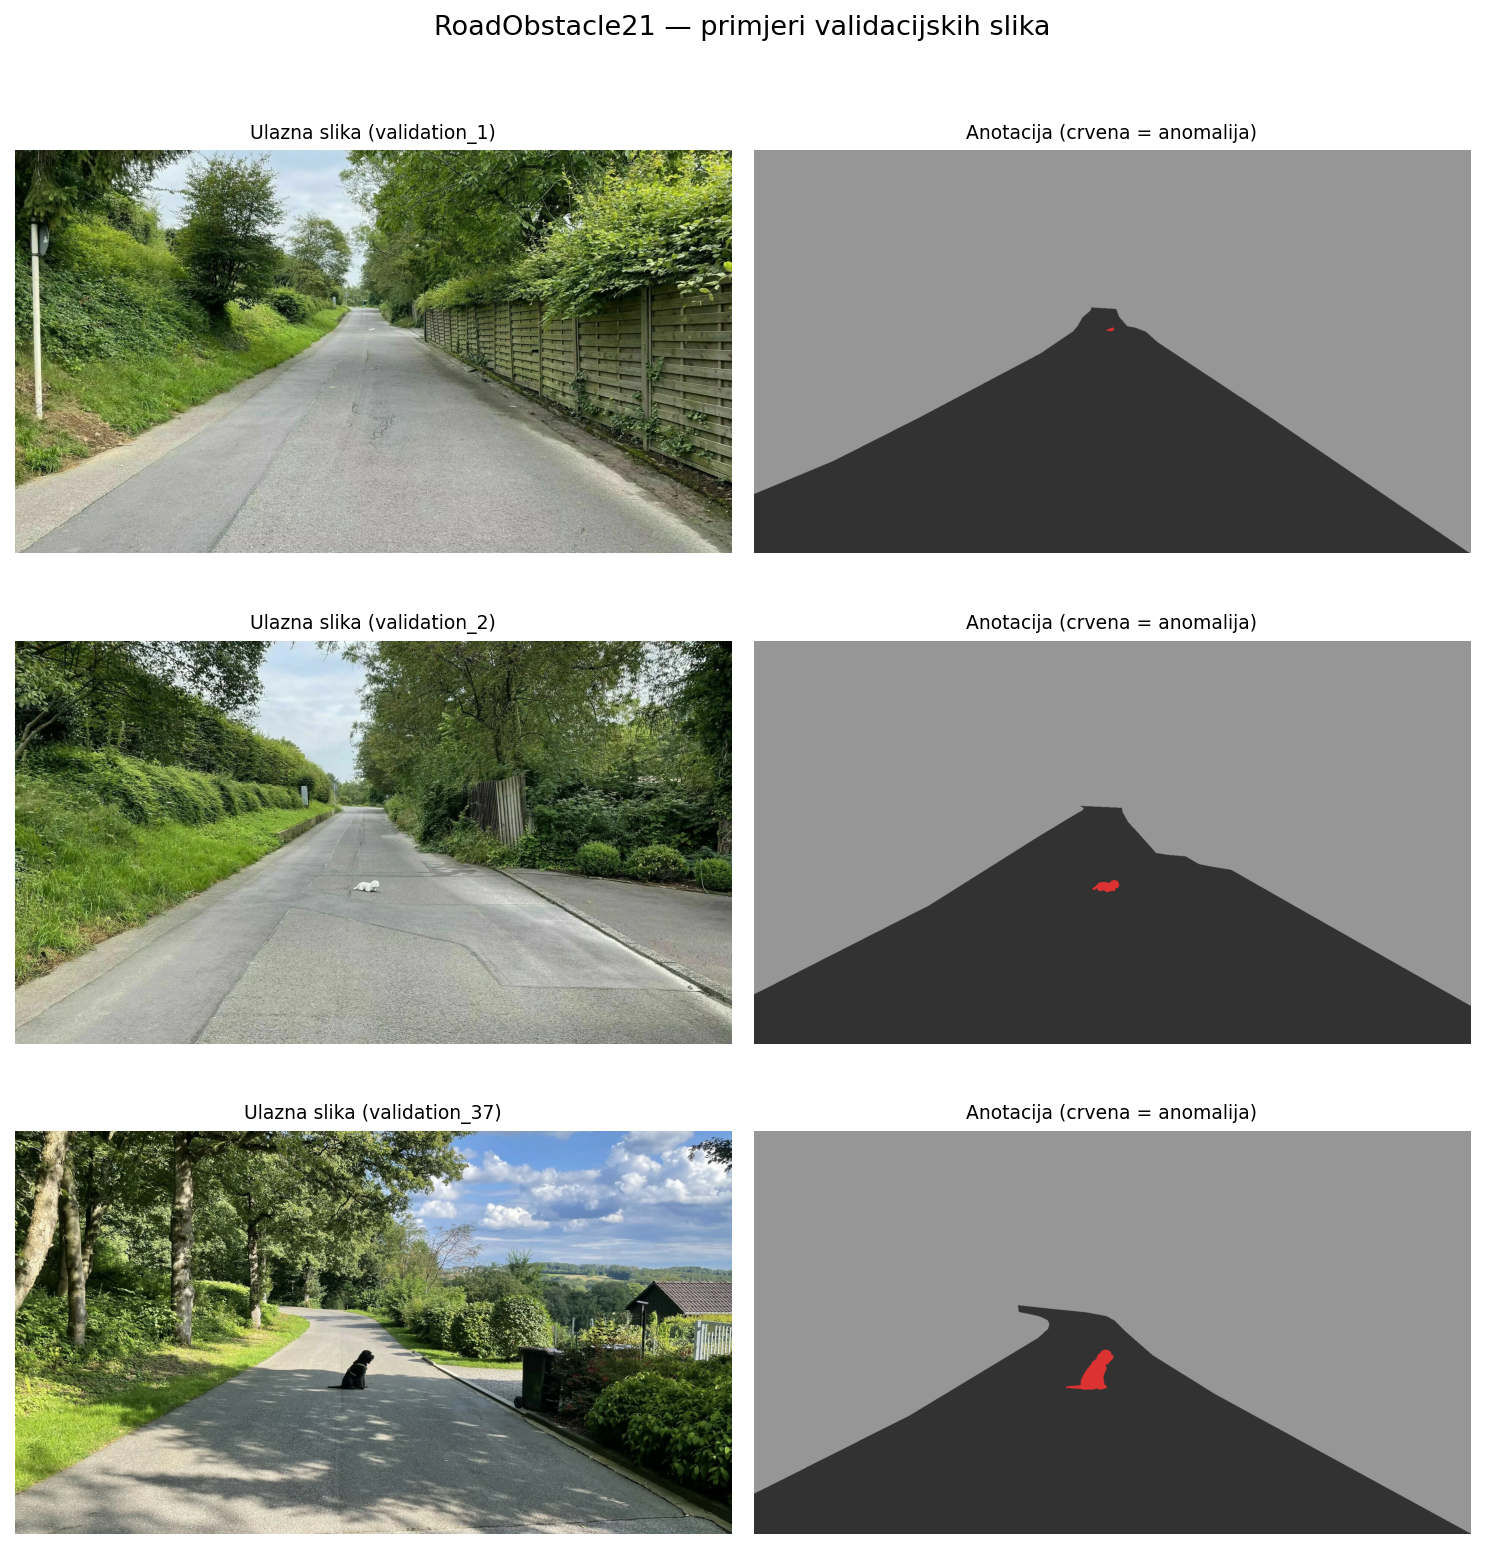
\includegraphics[width=\textwidth]{Figures/smiyc/smiyc_obstacle_examples.png}
	\caption{Primjeri iz RoadObstacle21 skupa podataka. Vidljive su prepreke na različitim vrstama podloge.}
	\label{fig:smiyc-obstacle}
\end{figure}

\subsection{Evaluacijski protokol i metrike}

Anotacijske maske koriste tri vrijednosti: 0 za normalne piksele, 1 za anomalne piksele i 255 za područja koja se ignoriraju pri evaluaciji. Evaluacija se provodi na dvije razine: pikselnoj i komponentnoj.

Na pikselnoj razini koriste se sljedeće metrike:
\begin{itemize}
	\item \textbf{AUPRC} (eng. \textit{Area Under the Precision-Recall Curve}) je površina ispod precision-recall krivulje. Primarna metrika za neuravnotežene skupove gdje je anomalnih piksela znatno manje od normalnih.
	\item \textbf{AUROC} (eng. \textit{Area Under the ROC Curve}) je površina ispod ROC krivulje. Mjeri sposobnost modela da razlikuje anomalne od normalnih piksela bez obzira na prag.
	\item \textbf{FPR95} je stopa lažno pozitivnih (eng. \textit{false positive rate}) pri odzivu (eng. \textit{recall}) od 95\%. Niže vrijednosti su bolje.
\end{itemize}

Na komponentnoj razini koriste se:
\begin{itemize}
	\item \textbf{sIoU} - srednji omjer presjeka i unije na razini segmenata (anomalnih komponenti)
	\item \textbf{F1} - harmonijska sredina preciznosti i odziva na razini detektiranih anomalnih objekata
\end{itemize}

Evaluacija na test skupovima provodi se putem Codabench platforme, budući da anotacije test slika nisu javno dostupne. Validacijski skupovi s javnim anotacijama korišteni su za lokalni razvoj i provjeru ispravnosti implementacije.



\section{Predobrada i augmentacije}
\label{sec:predobrada}

\subsection{Predobrada slika}

Sve slike su normalizirane srednjom vrijednosti i standardnom devijacijom izračunanim na skupu ImageNet: $\mu = (0.485, 0.456, 0.406)$ i $\sigma = (0.229, 0.224, 0.225)$ za RGB kanale. Ova normalizacija osigurava kompatibilnost s ResNet50 okosnicom predtreniranom na ImageNetu, čiji su konvolucijski filtri optimizirani za ulaze u tom rasponu vrijednosti.

Tijekom segmentacijskog dotreniranja, slike se izrezuju na veličinu 768$\times$768 piksela. Evaluacija se provodi na punoj rezoluciji ulaznih slika bez izrezivanja, pri čemu se dimenzije nadopunjuju na višekratnik od 16 piksela radi kompatibilnosti s koderom koji koristi operacije sažimanja s korakom 16.

\subsection{Augmentacije za segmentacijsko dotreniranje}

Augmentacije za segmentacijsko dotreniranje primjenjuju se sinkronizirano na sliku i odgovarajuću semantičku masku kako bi se očuvalo prostorno poravnanje anotacija. Koriste se sljedeće tehnike:

\begin{itemize}
	\item \textbf{Nasumično skaliranje} - slika i maska skaliraju se istim nasumičnim faktorom iz raspona $[0.5, 2.0]$
	\item \textbf{Nasumično izrezivanje} - iz skalirane slike izrezuje se isječak veličine 768$\times$768 piksela; područja izvan granica slike nadopunjuju se nulama za sliku i vrijednošću \texttt{ignore\_index} (255) za masku
	\item \textbf{Nasumično horizontalno zrcaljenje} - primjenjuje se s vjerojatnošću 0.5
	\item \textbf{Prilagodba boje} (eng. \textit{color jitter}) - nasumična promjena svjetline, kontrasta i zasićenosti primjenjuje se isključivo na sliku, ne na masku
\end{itemize}

\subsection{Augmentacije za SSL predtrening}

Augmentacijski skup za samonadzirani predtrening razlikuje se od onog za segmentaciju jer je cilj naučiti reprezentacije invarijantne na vizualne perturbacije, a ne očuvati prostornu strukturu. Koristi se standardni MoCo v2 augmentacijski protokol~\cite{chen2020improvedbaselinesmomentumcontrastive}:

\begin{itemize}
	\item \textbf{Nasumično izrezivanje i skaliranje} (eng. \textit{RandomResizedCrop}) - iz slike se izrezuje isječak veličine 224$\times$224 piksela s nasumičnom površinom iz raspona $[0.08, 1.0]$ originalne slike i nasumičnim omjerom stranica. Ovo je najvažnija augmentacija jer tjera model da uči semantiku iz djelomičnih pogleda.
	\item \textbf{Prilagodba boje} - nasumična promjena svjetline, kontrasta, zasićenosti i nijanse, primjenjuje se s vjerojatnošću 0.8
	\item \textbf{Nasumično pretvaranje u sivotone slike} - primjenjuje se s vjerojatnošću 0.2
	\item \textbf{Gaussovo zamagljivanje} - primjenjuje se s vjerojatnošću 0.5, s polumjerom jezgre 23 piksela i rasponom standardne devijacije $[0.1, 2.0]$
	\item \textbf{Nasumično horizontalno zrcaljenje} - primjenjuje se s vjerojatnošću 0.5
\end{itemize}

U standardnoj varijanti MoCo v2, oba pogleda na ulaznu sliku dobivaju se primjenom gore navedenih augmentacija na istu sliku. U temporalnoj varijanti, svaki pogled dolazi iz zasebnog okvira iste video sekvence, pri čemu se augmentacije primjenjuju na svaki okvir neovisno. Na taj način model mora naučiti reprezentacije koje su konzistentne i kroz vizualne perturbacije i kroz vremensku promjenu scene.




%-------------------------------------------------------------------------------
\chapter{Metodologija}
\label{pog:metodologija}

\section{Pregled sustava}
\label{sec:pregled_sustava}

Predloženi sustav sastoji se od triju uzastopnih faza prikazanih na slici~\ref{fig:pipeline}:

\begin{enumerate}
	\item \textbf{Samonadzirani predtrening} - ResNet50 okosnica predtrenira se 
	kontrastivnom metodom MoCo v2 na neoznačenim okvirima Cityscapes-Sequence 
	skupa. Ispituju se dvije varijante: standardna (pozitivni parovi su dvije 
	augmentacije iste slike) i temporalna (pozitivni parovi su dva okvira iz 
	iste video sekvence).
	\item \textbf{Segmentacijsko dotreniranje} - Predtrenirana okosnica 
	inicijalizira koder modela DeepLabV3+, koji se potom dotrenira 
	nadziranom semantičkom segmentacijom na označenom Cityscapes skupu.
	\item \textbf{Zaključivanje i ocjenjivanje anomalija} - Trenirani 
	segmentacijski model primjenjuje se na slike iz SMIYC benchmarka. 
	Logiti se transformiraju post-hoc funkcijama (MSP, MaxLogit, Energy) 
	u anomalne rezultate po pikselima koji se evaluiraju standardnim metrikama.
\end{enumerate}

\begin{figure}[H]
	\centering
	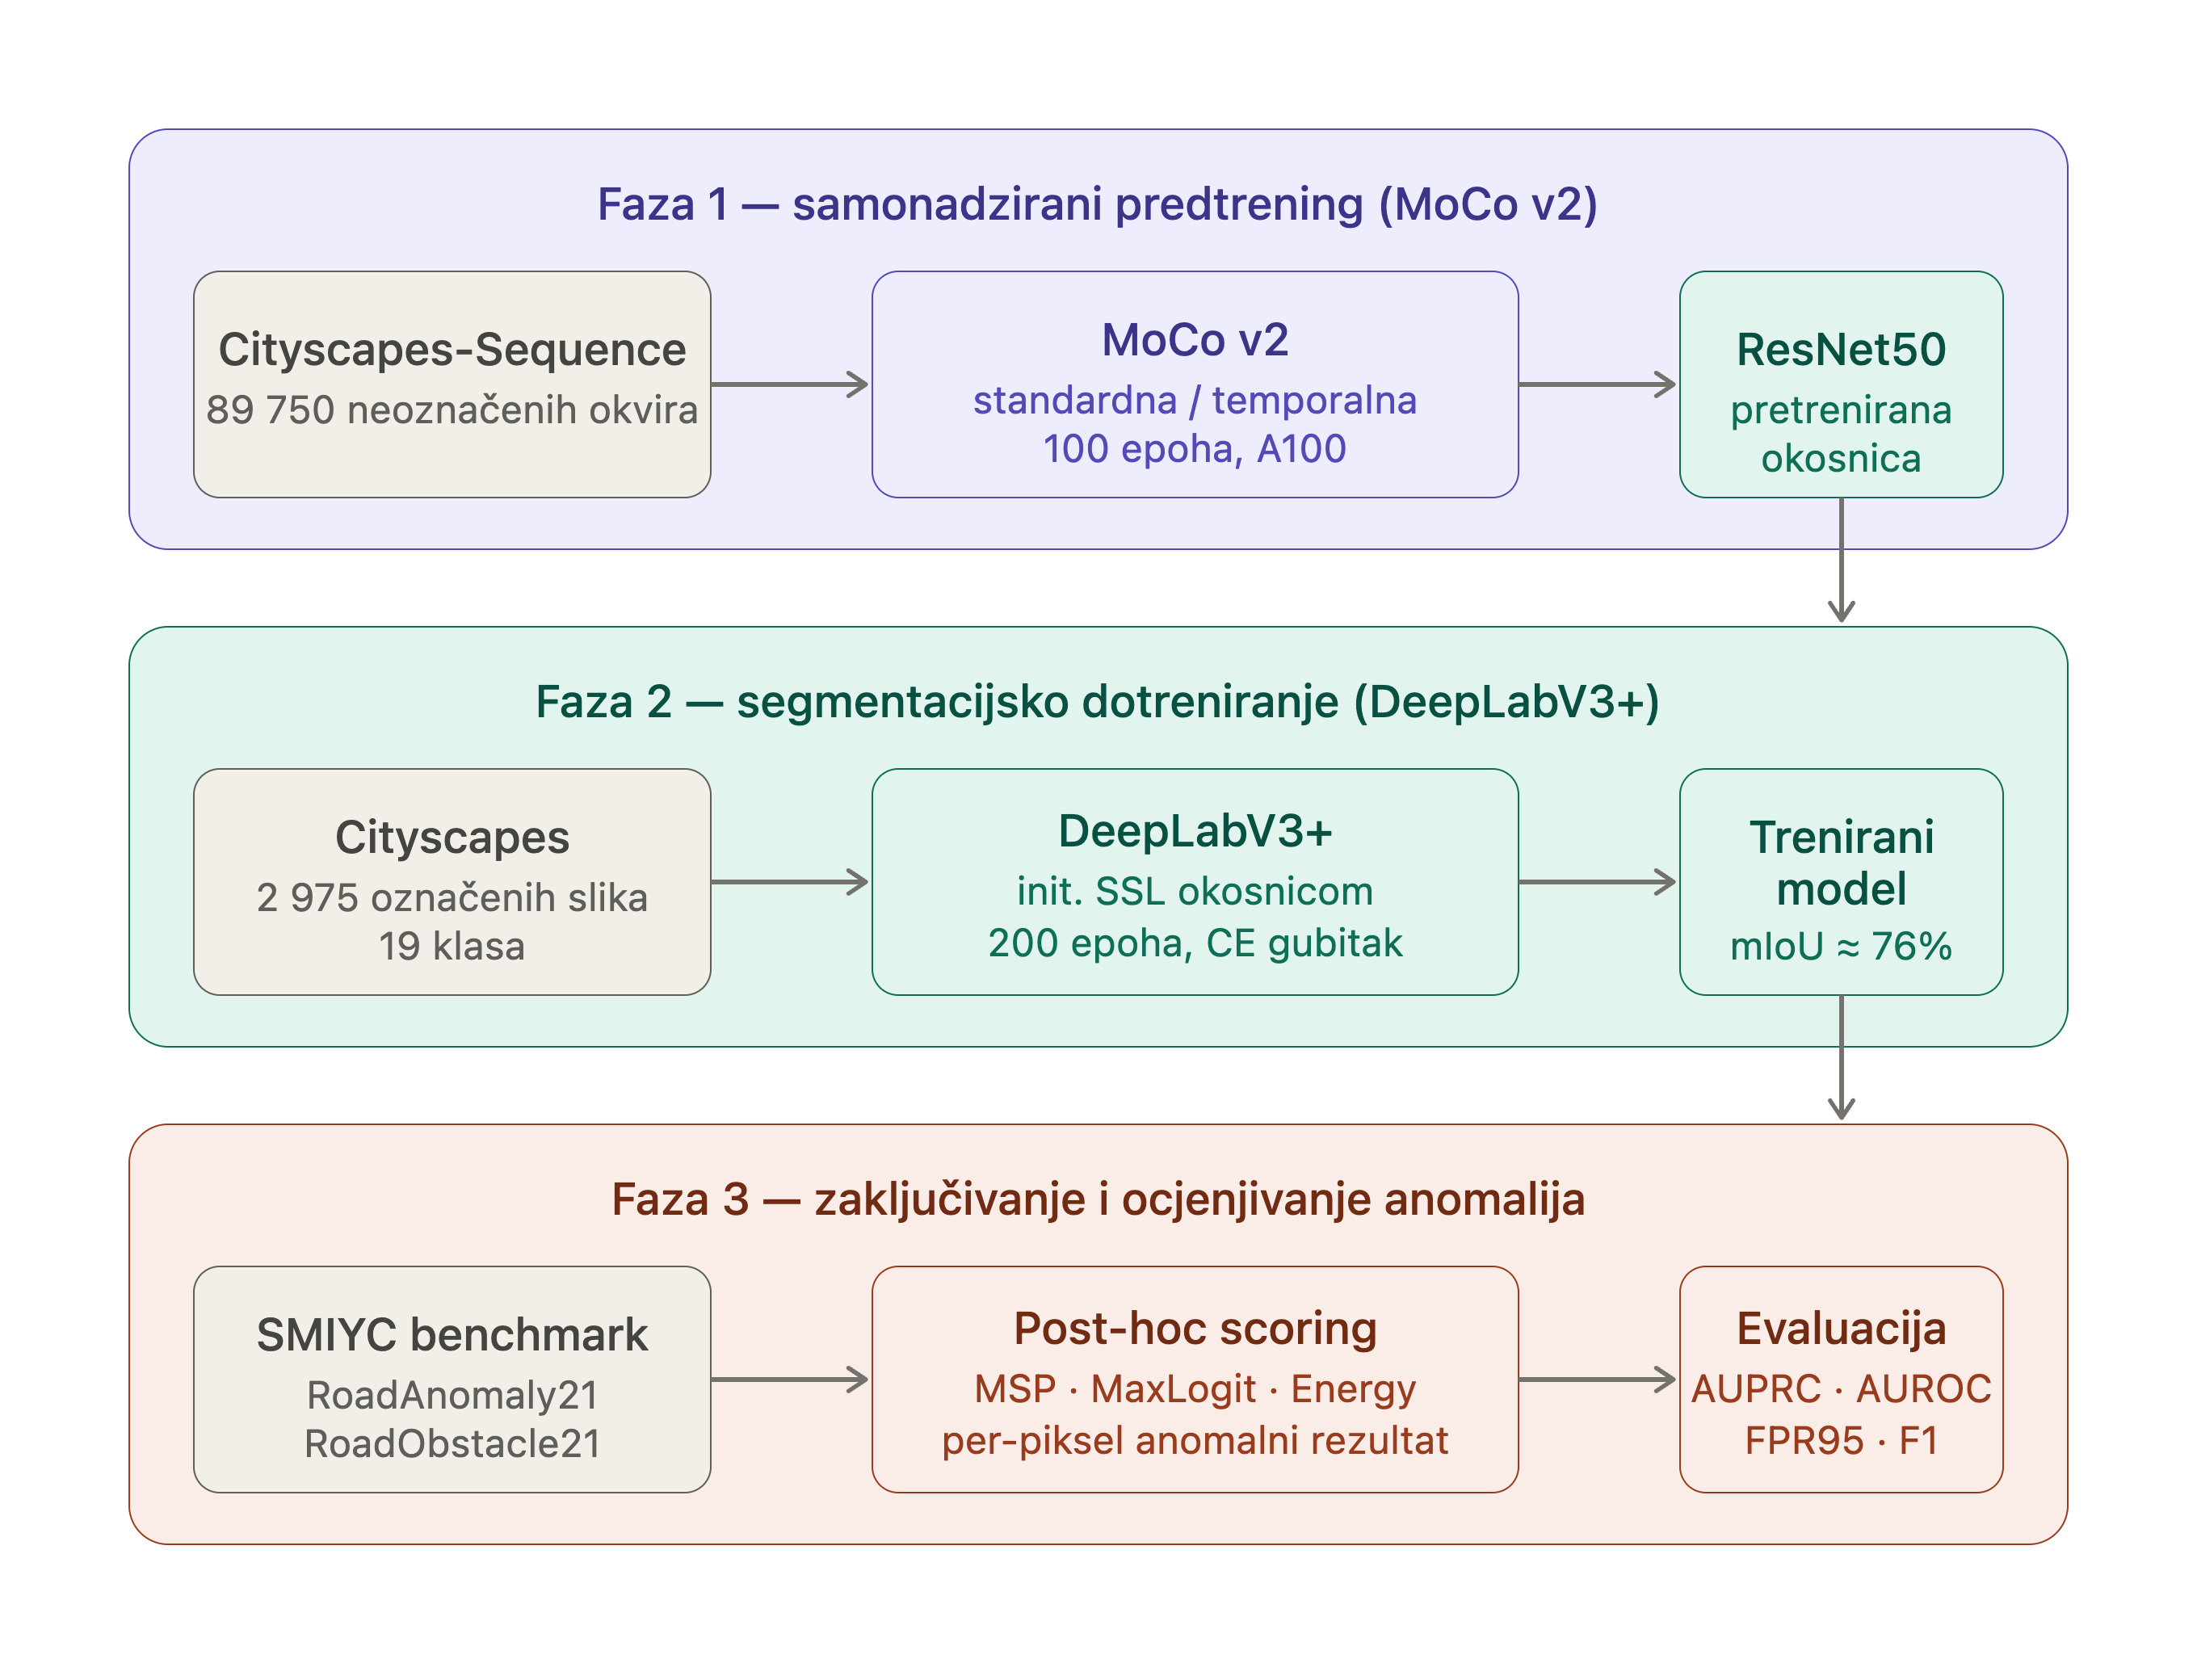
\includegraphics[width=\textwidth]{Figures/metodologija/pipeline_dijagram_sustava.png}
	\caption{Dijagram cijelog sustava: samonadzirani predtrening, 
		segmentacijsko dotreniranje i zaključivanje anomalija.}
	\label{fig:pipeline}
\end{figure}

Sva tri ispitana modela: osnovni model (ImageNet inicijalizacija bez SSL 
predtreninga), MoCo standard i MoCo temporal prolaze kroz identičnu drugu 
i treću fazu. Jedina razlika je inicijalizacija okosnice u prvoj fazi, 
što omogućuje poštenu usporedbu doprinosa svake strategije predtreninga.


\section{Samonadzirani predtrening}
\label{sec:ssl_predtrening}

\subsection{Standardna varijanta}

U standardnoj varijanti, pozitivni par za svaki uzorak čine dvije 
nasumične augmentacije iste slike. Okosnica ResNet50 inicijalizirana 
ImageNet težinama predtrenira se MoCo v2 algoritmom opisanim u 
odjeljku~\ref{sec:mocov2} na skupu Cityscapes-Sequence koji sadrži 
89\,750 neoznačenih okvira.

\subsection{Temporalna varijanta}
\label{sec:temporal-moco}

U temporalnoj varijanti, pozitivni par čine dva okvira iz iste video 
sekvence odabrana unutar maksimalnog vremenskog pomaka od 15 koraka:

\begin{equation}
	\mathbf{k} = f_{\theta_k}(\text{aug}(x_{t+\delta})), 
	\quad \delta \sim \mathcal{U}\{1, \ldots, 15\}
\end{equation}

gdje je $x_t$ sidro okvir, $x_{t+\delta}$ nasumično odabrani partner 
okvir iz istog isječka, a $\text{aug}(\cdot)$ standardni MoCo v2 
augmentacijski skup primijenjen neovisno na svaki okvir. Sve ostale 
komponente algoritma: momentum koder, pohrana negativnih primjera, 
InfoNCE gubitak, ostaju nepromijenjene.

Motivacija za ovu modifikaciju leži u temporalnoj strukturi prometnih 
scena: susjedni okviri prikazuju isti semantički sadržaj uz manje 
prostorne i fotometrijske varijacije uzrokovane kretanjem vozila. 
Temporalni signal tjera model da nauči reprezentacije robusne na 
promjene perspektive i osvjetljenja, što je korisno za detekciju 
anomalija.

\subsection{Hiperparametri predtreninga}

Oba modela predtreniraju se s jednakim hiperparametrima prikazanim 
u tablici~\ref{tab:ssl_hyperparams}.

\begin{table}[H]
	\centering
	\caption{Hiperparametri samonadziranog predtreninga.}
	\label{tab:ssl_hyperparams}
	\begin{tabular}{|l|l|}
		\hline
		\textbf{Hiperparametar} & \textbf{Vrijednost} \\
		\hline
		Okosnica            & ResNet50 (ImageNet init.) \\
		Skupna veličina     & 256 \\
		Broj epoha          & 100 \\
		Optimizator         & SGD, moment 0.9 \\
		Osnovna stopa učenja & 0.015 (kosinusni raspored) \\
		Raspad težina       & $10^{-4}$ \\
		Veličina pohrane    & 65536 \\
		Koeficijent momenta & 0.99 \\
		Temperatura $\tau$  & 0.2 \\
		Veličina isječka    & 224$\times$224 \\
		Maksimalni vremenski pomak & 15 (samo temporal) \\
		Mješovita preciznost & da (FP16) \\
		Sklopovlje          & NVIDIA A100 40 GB \\
		\hline
	\end{tabular}
\end{table}


\section{Segmentacijsko dotreniranje}
\label{sec:finetuning}

\subsection{Inicijalizacija}

Nakon samonadziranog predtreninga, težine kodera upita ($\theta_q$) 
učitavaju se kao inicijalizacija ResNet50 okosnice modela DeepLabV3+. 
Projekcijska glava MoCo v2 algoritma se odbacuje, koriste se samo 
težine okosnice. Segmentacijska glava (ASPP modul i dekoder) 
inicijalizira se nasumično. Cijeli model dotrenira se \textit{end-to-end} 
bez zamrzavanja ikojeg dijela.

Osnovni model (bez SSL predtreninga) inicijalizira se standardnim 
ImageNet težinama, što je uobičajeni postupak za semantičku 
segmentaciju~\cite{he2016resnet}.

\subsection{Hiperparametri dotreniranja}

\begin{table}[H]
	\centering
	\caption{Hiperparametri segmentacijskog dotreniranja.}
	\label{tab:seg_hyperparams}
	\begin{tabular}{|l|l|}
		\hline
		\textbf{Hiperparametar} & \textbf{Vrijednost} \\
		\hline
		Optimizator         & SGD, moment 0.9 \\
		Osnovna stopa učenja & 0.01 (polinomijalni raspored, $p = 0.9$) \\
		Raspad težina       & $5 \times 10^{-4}$ \\
		Skupna veličina     & 8 \\
		Broj epoha          & 200 \\
		Veličina isječka    & 768$\times$768 \\
		Funkcija gubitka    & unakrsna entropija, \texttt{ignore\_index=255} \\
		Mješovita preciznost & da (FP16) \\
		Sklopovlje          & NVIDIA A100 40 GB \\
		\hline
	\end{tabular}
\end{table}

Augmentacije korištene tijekom dotreniranja opisane su u 
odjeljku~\ref{sec:predobrada}.


\section{Zaključivanje i ocjenjivanje anomalija}
\label{sec:anomaly_metoda}

\subsection{Princip rada}

Trenirani segmentacijski model primjenjuje se na slike iz SMIYC 
benchmarka bez ikakvih izmjena težina. Za svaki ulazni piksel model 
producira vektor logita $\mathbf{z} \in \mathbb{R}^{19}$. Pikseli 
koji prikazuju anomalne objekte očekivano daju nesigurnu distribuciju 
po klasama (niske maksimalne logite, visoku entropiju), dok pikseli 
poznate scene daju sigurnu predikciju jedne klase.

\subsection{Implementacija ocjenjivanja}

Tri post-hoc funkcije za ocjenu anomalija opisane u 
odjeljku~\ref{sec:anomaly_detection} primjenjuju se neovisno na 
svaki piksel. Izlaz svake funkcije je karta anomalija iste prostorne 
rezolucije kao ulazna slika. Slike koje nisu višekratnik od 16 
piksela nadopunjuju se refleksijskim nadopunjavanjem (eng. 
\textit{reflect padding}) prije zaključivanja, a karte anomalija 
se potom orezuju na originalnu rezoluciju.

\subsection{Evaluacijski protokol}

Evaluacija se provodi na dvama podskupovima SMIYC benchmarka: 
RoadAnomaly21 i RoadObstacle21. Za svaki model i svaku funkciju 
ocjenjivanja izračunavaju se metrike opisane u 
odjeljku~\ref{sec:smiyc}: AUPRC, AUROC i FPR95 na razini piksela 
te sIoU i F1 na razini komponenti. Službena evaluacija na test 
skupovima provedena je putem Codabench platforme.




%-------------------------------------------------------------------------------
\chapter{Rezultati i rasprava}
\label{pog:rezultati_i_rasprava}

Ovo poglavlje prikazuje rezultate triju ispitanih modela na zadatku
detekcije anomalija u prometnim scenama. Najprije se prikazuju
krivulje gubitka samonadziranog predtreninga, zatim rezultati
segmentacijskog dotreniranja, a potom glavni rezultati detekcije
anomalija na SMIYC benchmarku, lokalno na validacijskom skupu te
službeno na test skupu putem Codabench platforme.


\section{Samonadzirani predtrening}
\label{sec:rezultati_ssl}

\begin{figure}[H]
	\centering
	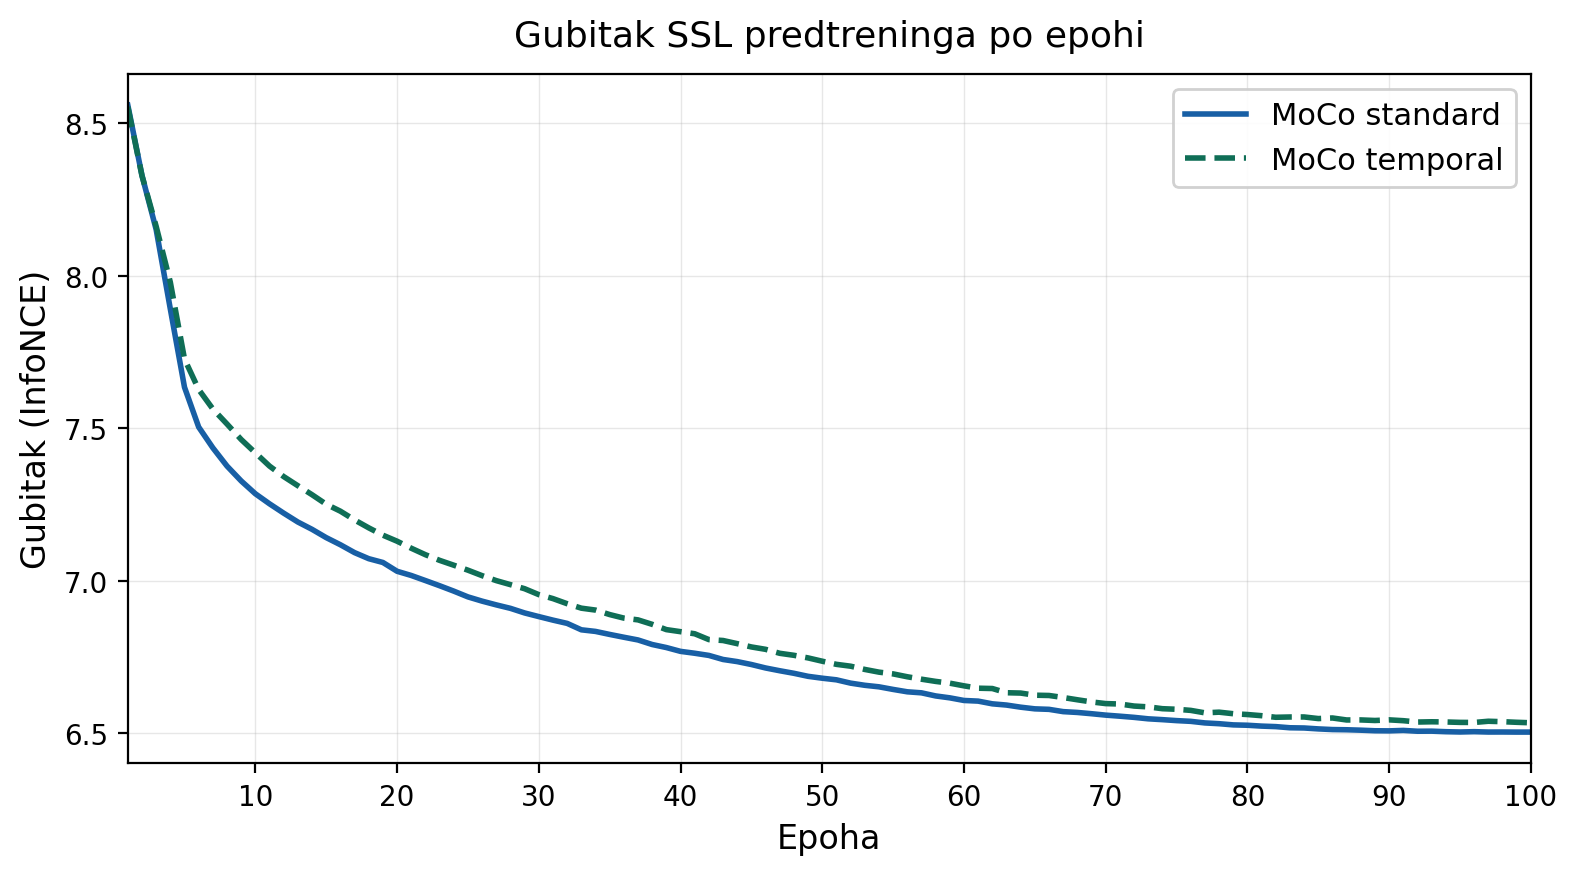
\includegraphics[width=0.9\textwidth]{Figures/loss/ssl_epoch_loss.png}
	\caption{Gubitak MoCo v2 predtreninga po epohi za standardnu i
		temporalnu varijantu.}
	\label{fig:ssl_loss}
\end{figure}

Slika~\ref{fig:ssl_loss} prikazuje krivulje gubitka InfoNCE kroz
100 epoha samonadziranog predtreninga za obje varijante. Obje
krivulje kreću s visokim početnim gubitkom od oko 8{,}5, što je
niže od teorijskog maksimuma $\log(65537) \approx 11{,}1$ koji bi
odgovarao potpuno nasumičnim reprezentacijama. Niža početna
vrijednost posljedica je ImageNet inicijalizacije okosnice koja već
kodira semantički korisne vizualne značajke.

Gubitak monotono opada kroz cijelo treniranje kod obje varijante,
bez znakova nestabilnosti ili kolapsa reprezentacija. Do epohe 100
oba modela konvergiraju prema vrijednosti od oko 6{,}5. Međusobna
razlika između standardne i temporalne varijante je zanemariva
(manja od 0{,}1), što ukazuje da zamjena pozitivnih parova od
augmentacija iste slike na susjedne okvire video sekvence ne
narušava stabilnost kontrastivnog učenja.


\section{Rezultati segmentacijskog dotreniranja}
\label{sec:rezultati_segmentacija}

Tablica~\ref{tab:miou} prikazuje postignute vrijednosti mIoU na
Cityscapes validacijskom skupu za sva tri modela. Sva tri modela
postižu usporedive vrijednosti, što je preduvjet za poštenu
usporedbu u zadatku detekcije anomalija, razlike u AUPRC-u ne
mogu se pripisati općoj kvaliteti segmentacijskog modela, već
isključivo strategiji inicijalizacije okosnice.

\begin{table}[H]
	\centering
	\caption{Rezultati semantičke segmentacije na Cityscapes
		validacijskom skupu.}
	\label{tab:miou}
	\begin{tabular}{|l|c|c|}
		\hline
		\textbf{Model} & \textbf{Inicijalizacija okosnice} & \textbf{mIoU} \\
		\hline
		Osnovni model & ImageNet                      & 76{,}91\% \\
		MoCo standard & ImageNet + SSL (image)         & 76{,}81\% \\
		MoCo temporal & ImageNet + SSL (temporal)      & 76{,}57\% \\
		\hline
	\end{tabular}
\end{table}

Razlike između modela su unutar $\pm 0{,}35$ postotnih bodova, što
odgovara tipičnom šumu evaluacije pri treniranju semantičke
segmentacije. Može se zaključiti da samonadzirani predtrening nije
narušio sposobnost modela za segmentaciju poznatih klasa.

\begin{figure}[H]
	\centering
	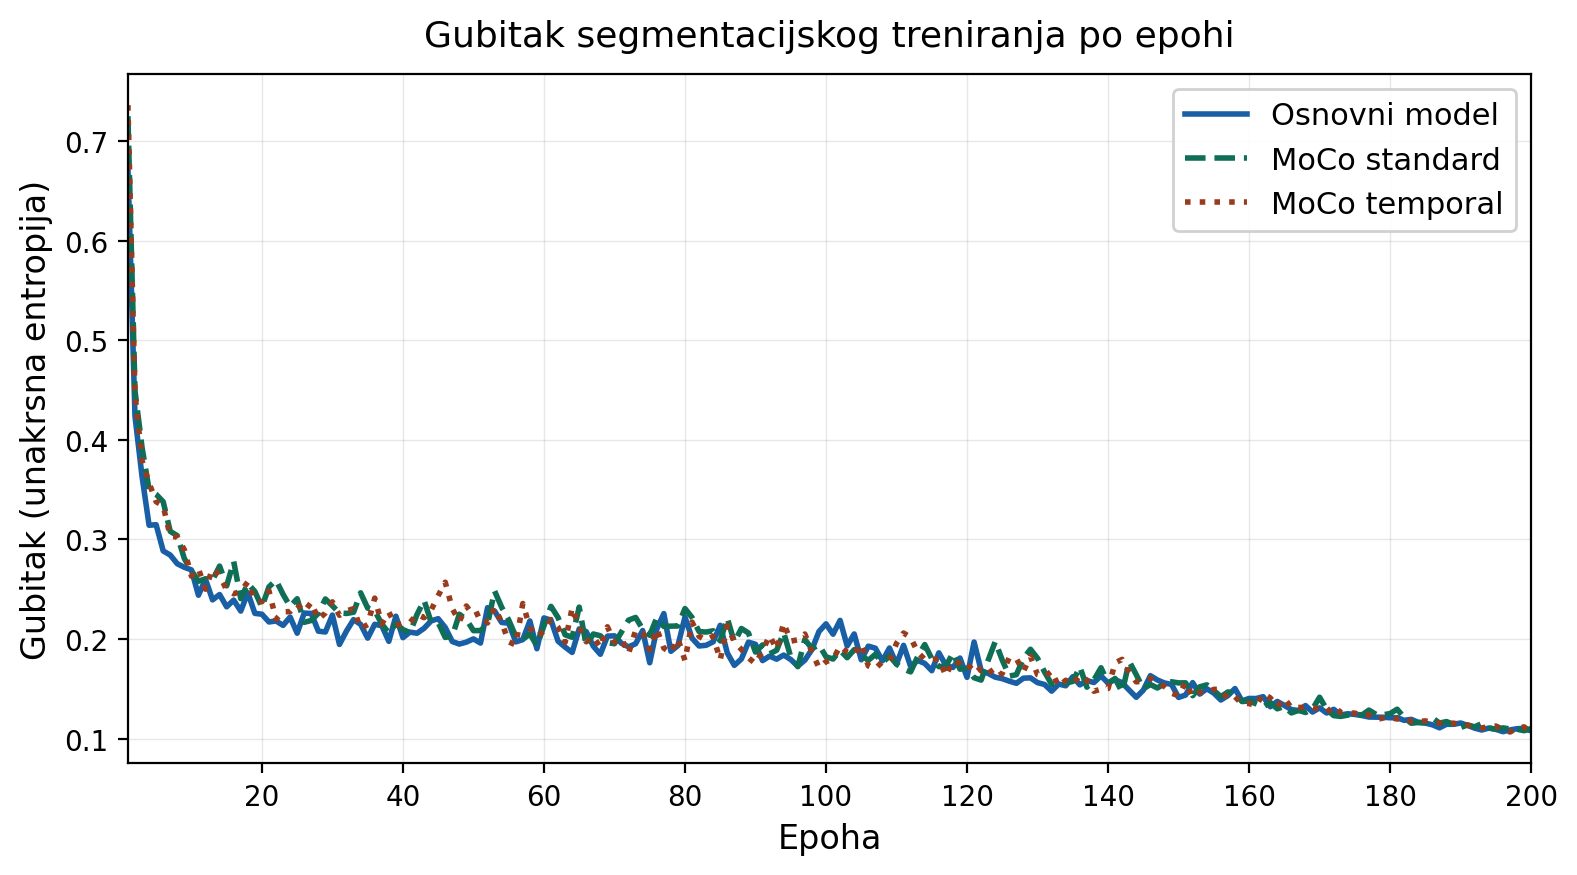
\includegraphics[width=0.9\textwidth]{Figures/loss/seg_epoch_loss.png}
	\caption{Gubitak segmentacijskog dotreniranja po epohi za sva tri
		modela.}
	\label{fig:seg_loss}
\end{figure}

\begin{figure}[H]
	\centering
	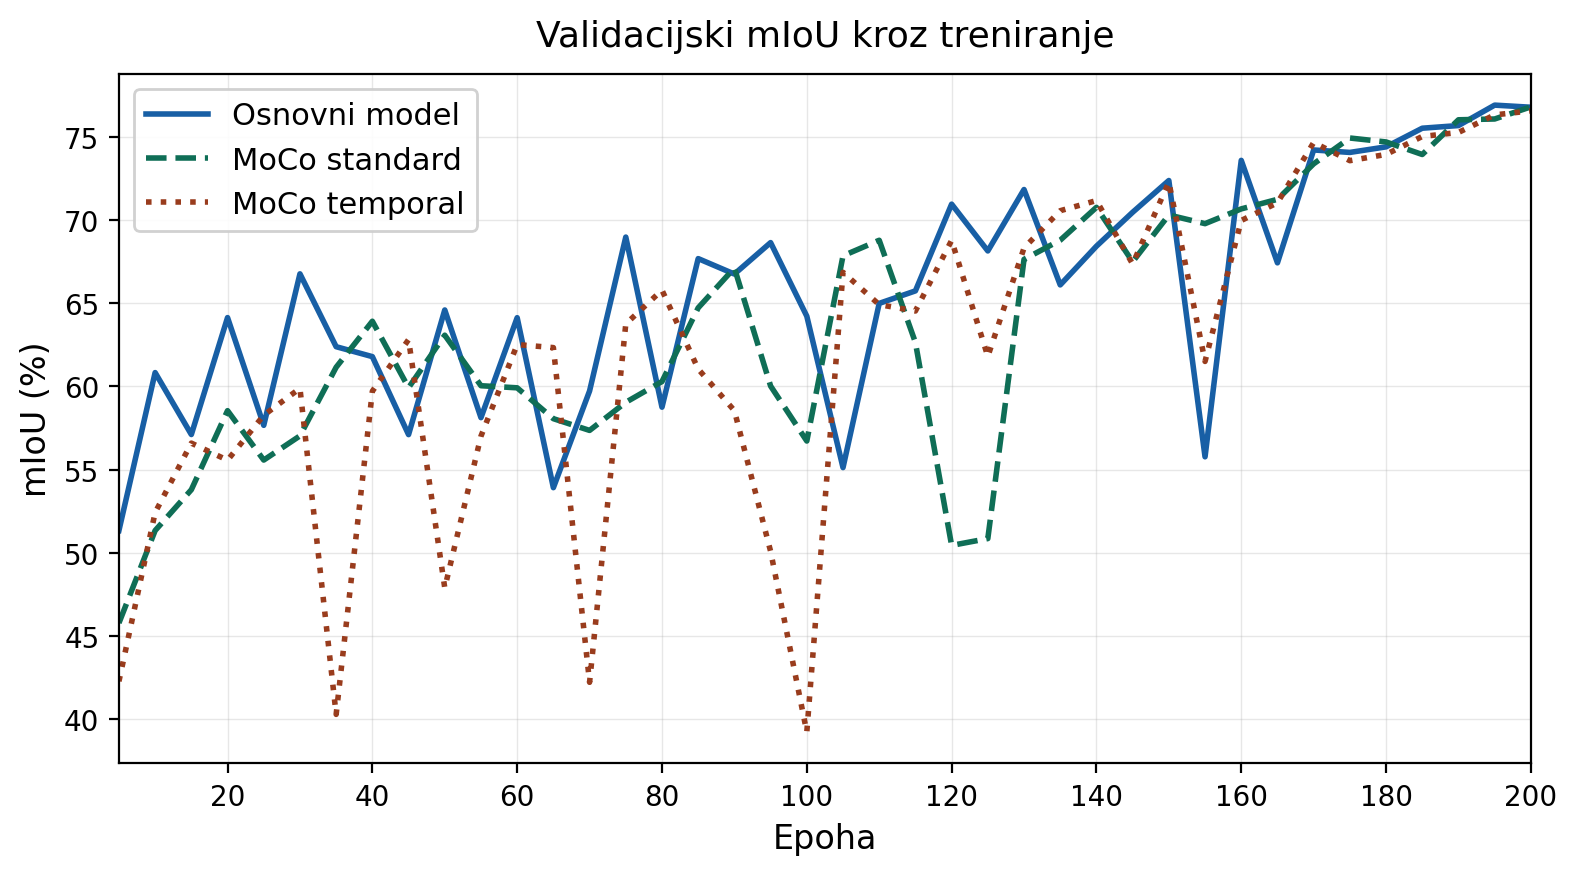
\includegraphics[width=0.9\textwidth]{Figures/loss/seg_val_miou.png}
	\caption{Validacijski mIoU kroz 200 epoha segmentacijskog
		treniranja.}
	\label{fig:seg_miou}
\end{figure}

Krivulje gubitka (slika~\ref{fig:seg_loss}) pokazuju karakteristični
obrazac segmentacijskog dotreniranja. Sva tri modela kreću s početnim
gubitkom između 0{,}7 i 0{,}9 i brzo opadaju u prvih 20--30 epoha,
nakon čega konvergiraju prema stabilnoj vrijednosti ispod 0{,}3.
Strmiji pad u ranim epohama posljedica je polinomijalnog rasporeda
stope učenja koji drži relativno visoku stopu na početku treniranja.
Razlike između triju krivulja minimalne su kroz cijelo treniranje,
što potvrđuje da strategija inicijalizacije okosnice ne utječe
značajno na dinamiku segmentacijskog dotreniranja.

Krivulje validacijskog mIoU (slika~\ref{fig:seg_miou}) pokazuju
stabilan rast od prvih mjerenja oko epohe 5 (mIoU $\approx$
40--50\%) prema konačnim vrijednostima oko 76--77\%. Sve tri
krivulje konvergiraju gotovo identično, razlika između najboljeg i
najlošijeg modela na kraju treniranja iznosi samo 0{,}34 postotna
boda. Blago valoviti karakter krivulja u kasnijim epohama rezultat
je padajuće stope učenja, što uzrokuje male oscilacije pri evaluaciji
na validacijskom skupu. Ovi grafovi vizualno potvrđuju temeljnu
pretpostavku eksperimenta: sva tri modela postigla su usporedivu
razinu segmentacijske sposobnosti, što je nužan uvjet za
interpretaciju razlika u detekciji anomalija kao posljedice
strategije predtreninga, a ne opće kvalitete modela.


\section{Rezultati detekcije anomalija}
\label{sec:rezultati_anomalije}

\subsection{Evaluacija na validacijskom skupu}

Tablice~\ref{tab:val_anomaly} i~\ref{tab:val_obstacle} prikazuju
rezultate lokalne evaluacije na javno dostupnim validacijskim
skupovima SMIYC benchmarka (10 slika RoadAnomaly21, 30 slika
RoadObstacle21). Prikazuju se sve tri funkcije ocjenjivanja
anomalija.

\begin{table}[H]
	\centering
	\caption{Rezultati na RoadAnomaly21 validacijskom skupu
		(10 slika).}
	\label{tab:val_anomaly}
	\begin{tabular}{|l|l|c|c|c|}
		\hline
		\textbf{Model} & \textbf{Metoda} & \textbf{AUPRC} &
		\textbf{AUROC} & \textbf{FPR95} \\
		\hline
		\multirow{3}{*}{Osnovni model}
		& MSP      & 40{,}09\% & 80{,}55\% & 49{,}70\% \\
		& MaxLogit & 45{,}85\% & 83{,}01\% & 50{,}80\% \\
		& Energy   & 46{,}34\% & 83{,}22\% & 50{,}17\% \\
		\hline
		\multirow{3}{*}{MoCo standard}
		& MSP      & 38{,}23\% & 75{,}56\% & 62{,}40\% \\
		& MaxLogit & 40{,}70\% & 75{,}63\% & 73{,}12\% \\
		& Energy   & 40{,}42\% & 75{,}51\% & 72{,}94\% \\
		\hline
		\multirow{3}{*}{MoCo temporal}
		& MSP      & 44{,}36\% & 83{,}86\% & 49{,}48\% \\
		& MaxLogit & 41{,}72\% & 82{,}00\% & 49{,}48\% \\
		& Energy   & 39{,}02\% & 80{,}68\% & 51{,}83\% \\
		\hline
	\end{tabular}
\end{table}

\begin{table}[H]
	\centering
	\caption{Rezultati na RoadObstacle21 validacijskom skupu
		(30 slika).}
	\label{tab:val_obstacle}
	\begin{tabular}{|l|l|c|c|c|}
		\hline
		\textbf{Model} & \textbf{Metoda} & \textbf{AUPRC} &
		\textbf{AUROC} & \textbf{FPR95} \\
		\hline
		\multirow{3}{*}{Osnovni model}
		& MSP      & 11{,}31\% & 93{,}99\% & 20{,}64\% \\
		& MaxLogit & 32{,}32\% & 94{,}86\% & 21{,}31\% \\
		& Energy   & 40{,}88\% & 95{,}01\% & 21{,}32\% \\
		\hline
		\multirow{3}{*}{MoCo standard}
		& MSP      &  8{,}51\% & 94{,}07\% & 25{,}02\% \\
		& MaxLogit & 18{,}42\% & 94{,}75\% & 24{,}36\% \\
		& Energy   & 24{,}85\% & 94{,}92\% & 24{,}42\% \\
		\hline
		\multirow{3}{*}{MoCo temporal}
		& MSP      & 37{,}95\% & 97{,}25\% & 11{,}26\% \\
		& MaxLogit & 49{,}95\% & 97{,}63\% & 11{,}44\% \\
		& Energy   & 49{,}01\% & 97{,}62\% & 11{,}56\% \\
		\hline
	\end{tabular}
\end{table}

\subsection{Službena evaluacija na test skupu}

Tablica~\ref{tab:test_results} prikazuje službene rezultate
evaluacije na SMIYC test skupu dobivene putem Codabench platforme.
Prikazuje se Energy funkcija ocjenjivanja kao primarna metoda te
pikselne i komponentne metrike.

\begin{table}[H]
	\centering
	\caption{Službeni rezultati na SMIYC test skupu (Energy
		scoring).}
	\label{tab:test_results}
	\begin{tabular}{|l|c|c|c|c|c|}
		\hline
		\multirow{2}{*}{\textbf{Model}} &
		\multicolumn{5}{c|}{\textbf{RoadAnomaly21 test
				(100 slika)}} \\
		\cline{2-6}
		& \textbf{AUPRC} & \textbf{AUROC} & \textbf{FPR95} &
		\textbf{sIoU} & \textbf{F1} \\
		\hline
		Osnovni model & 34{,}97\% & 78{,}89\% & 58{,}34\% &
		18{,}36\% & 5{,}69\% \\
		MoCo standard & 30{,}86\% & 75{,}29\% & 68{,}40\% &
		15{,}84\% & 4{,}48\% \\
		MoCo temporal & 28{,}45\% & 72{,}38\% & 73{,}10\% &
		17{,}47\% & 5{,}63\% \\
		\hline
		\multirow{2}{*}{\textbf{Model}} &
		\multicolumn{5}{c|}{\textbf{RoadObstacle21 test
				(327 slika)}} \\
		\cline{2-6}
		& \textbf{AUPRC} & \textbf{AUROC} & \textbf{FPR95} &
		\textbf{sIoU} & \textbf{F1} \\
		\hline
		Osnovni model &  6{,}85\% & 89{,}79\% & 33{,}67\% &
		8{,}79\% & 4{,}94\% \\
		MoCo standard &  4{,}44\% & 87{,}50\% & 40{,}41\% &
		10{,}72\% & 6{,}43\% \\
		MoCo temporal &  7{,}34\% & 90{,}03\% & 40{,}30\% &
		18{,}77\% & 8{,}56\% \\
		\hline
	\end{tabular}
\end{table}


\section{Rasprava}
\label{sec:rasprava}

\subsection{Utjecaj samonadziranog predtreninga}

Rezultati pokazuju da samonadzirani predtrening MoCo v2 algoritmom
na Cityscapes-Sequence skupu ne donosi konzistentno poboljšanje
detekcije anomalija u odnosu na osnovni model s ImageNet
inicijalizacijom. Analiza rezultata otkriva nekoliko zanimljivih
obrazaca.

\textbf{MoCo standard slabiji je od osnovnog modela na svim
	skupovima.} Na RoadAnomaly21 test skupu MoCo standard postiže
AUPRC od 30{,}86\%, u usporedbi s 34{,}97\% osnovnog modela.
Sličan obrazac vidljiv je i na RoadObstacle21 (4{,}44\% nasuprot
6{,}85\%). Ovaj nalaz sugerira da kontrastivno učenje na razini
slike na domenski specifičnom skupu od 89\,750 okvira nije
dostatno da poboljša ImageNet inicijalizaciju za zadatak detekcije
anomalija, štoviše može je blago narušiti specijalizacijom
okosnice na uske vizualne karakteristike prometnih scena.

\textbf{MoCo temporal konzistentno nadmašuje MoCo standard.}
Na RoadObstacle21 test skupu MoCo temporal postiže AUPRC od
7{,}34\%, što je za 2{,}9 postotnih bodova bolje od MoCo standarda
(4{,}44\%) i blago bolje od osnovnog modela (6{,}85\%). Dosljedniji
napredak vidljiv je u komponentnim metrikama: sIoU MoCo temporala
(18{,}77\%) značajno je viši od osnovnog modela (8{,}79\%) i MoCo
standarda (10{,}72\%). Ovaj nalaz podupire hipotezu da temporalni
signal pruža korisniji nadzorni signal od augmentacija iste slike
za učenje reprezentacija robusnih na prepreke u prometnim scenama.

\textbf{RoadAnomaly21 i RoadObstacle21 pokazuju suprotne trendove.}
Na RoadAnomaly21 osnovni model ostaje najuspješniji, dok MoCo
temporal lagano zaostaje. Vjerojatno objašnjenje leži u prirodi
anomalija: RoadAnomaly21 sadrži vizualno raznolike objekte
prikupljene s interneta koji su daleko od prometne domene, pa
specijalizacija okosnice na Cityscapes domenu može štetiti
generalizaciji na takve OOD uzorke. RoadObstacle21, s druge strane
sadrži objekte postavljene na prometne scene snimljene iz automobila, domenu blisku Cityscapes-Sequence skupu za predtrening.

\subsection{Raskorak između validacijskih i test rezultata}

Primjetan je značajan raskorak između rezultata na validacijskom
skupu i službenih test rezultata. Na primjer, MoCo temporal postiže
AUPRC od 49{,}01\% na RoadObstacle21 validacijskom skupu, ali samo
7{,}34\% na test skupu. Ovaj raskorak posljedica je male veličine
validacijskog skupa (30 slika) koja ne može reprezentativno
obuhvatiti raznolikost punog test skupa (327 slika). Zaključke o
performansama modela stoga je potrebno temeljiti primarno na
službenim test rezultatima.

\subsection{Ograničenja i smjernice za buduća istraživanja}

Rezultati ovog rada ukazuju na nekoliko ograničenja trenutnog
pristupa. Kao prvo, 100 epoha samonadziranog predtreninga na
89\,750 okvira relativno je kratko u usporedbi s tipičnim SSL
predtreninzima koji zahtijevaju 200--800 epoha na znatno većim
skupovima. Kao drugo, korištene post-hoc funkcije ocjenjivanja
anomalija nisu optimizirane za detekciju anomalija, specijalizirane
metode poput PEBAL ili Mask2Anomaly tipično postižu znatno više
apsolutne vrijednosti AUPRC. Treće, MoCo v2 dizajniran je za
višestruke grafičke procesore sa Shuffle BN mehanizmom; korištena
implementacija s jednim grafičkim procesorom mogla je ograničiti
kvalitetu naučenih reprezentacija.

Buduća istraživanja mogla bi ispitati duži predtrening, veće skupove
(npr. BDD100K ili nuScenes), kombinirani pristup koji spaja SSL
predtrening s outlier exposure dotreniranjem, te primjenu novijih
SSL metoda poput DINO ili MAE prilagođenih za segmentacijske zadatke.

\subsection{Kvalitativna analiza}

Slike~\ref{fig:qual_anomaly} i~\ref{fig:qual_obstacle} prikazuju
primjere anomalnih karata ocjenjivanja Energy funkcijom za odabrane
primjere iz SMIYC validacijskog skupa, a slika~\ref{fig:qual_scoring}
uspoređuje sve tri funkcije ocjenjivanja na Cityscapes scenama s
digitalno ubačenim anomalijama.

\begin{figure}[H]
	\centering
	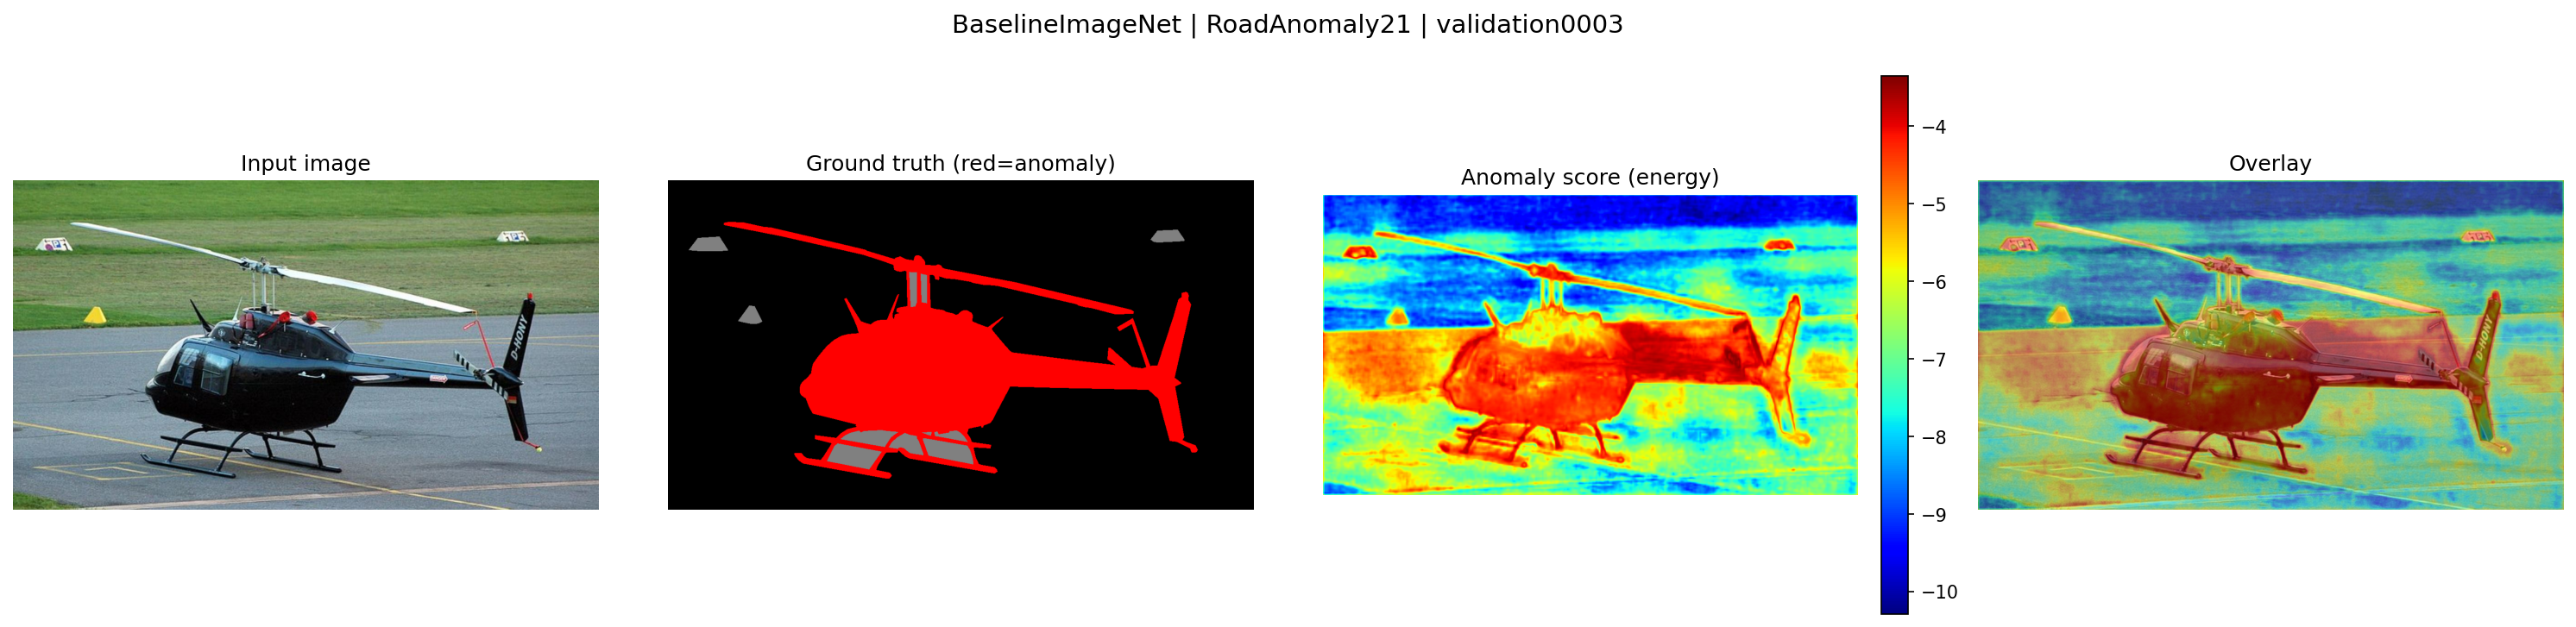
\includegraphics[width=\textwidth]{Figures/kvalitativno/BaselineImageNet_RoadAnomaly21_validation0003_energy.png}
	\vspace{2mm}
	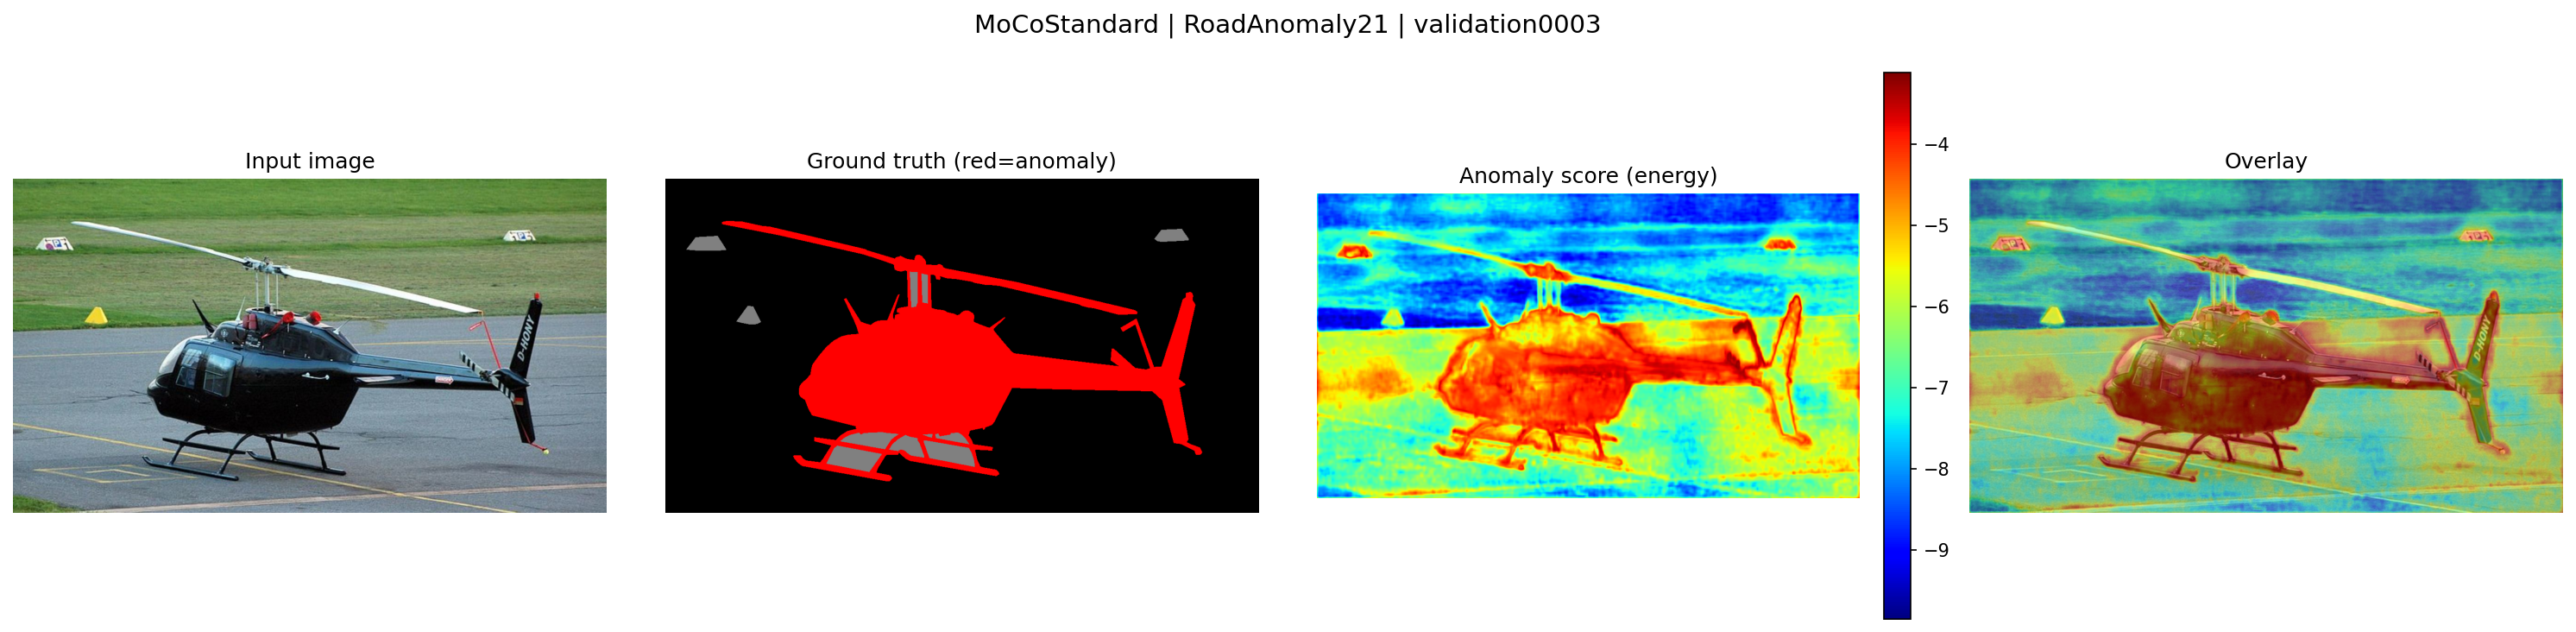
\includegraphics[width=\textwidth]{Figures/kvalitativno/MoCoStandard_RoadAnomaly21_validation0003_energy.png}
	\caption{Usporedba osnovnog modela (gore) i MoCo standard modela
		(dolje) na primjeru helikoptera iz RoadAnomaly21
		validacijskog skupa (Energy scoring). Oba modela
		uspješno detektiraju helikopter kao anomaliju (topla
		boja), ali MoCo standard pokazuje niže apsolutne
		vrijednosti energetskog rezultata i više lažno pozitivnih
		piksela na pozadinskim površinama.}
	\label{fig:qual_anomaly}
\end{figure}

\begin{figure}[H]
	\centering
	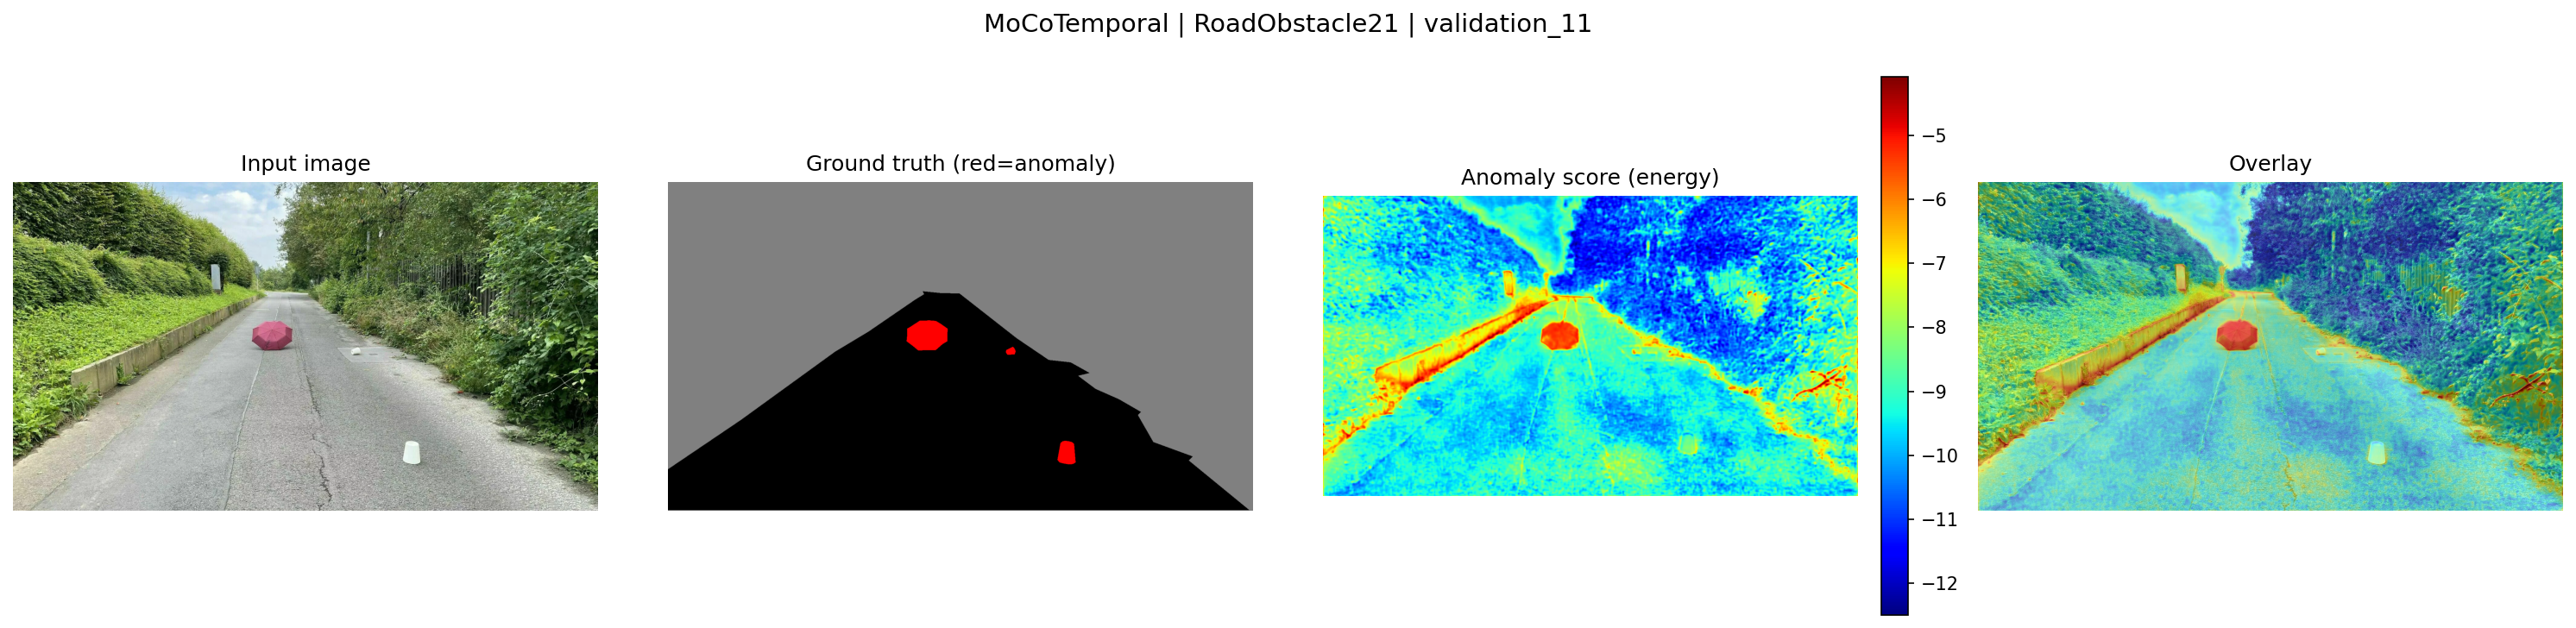
\includegraphics[width=\textwidth]{Figures/kvalitativno/MoCoTemporal_RoadObstacle21_validation_11_energy.png}
	\vspace{2mm}
	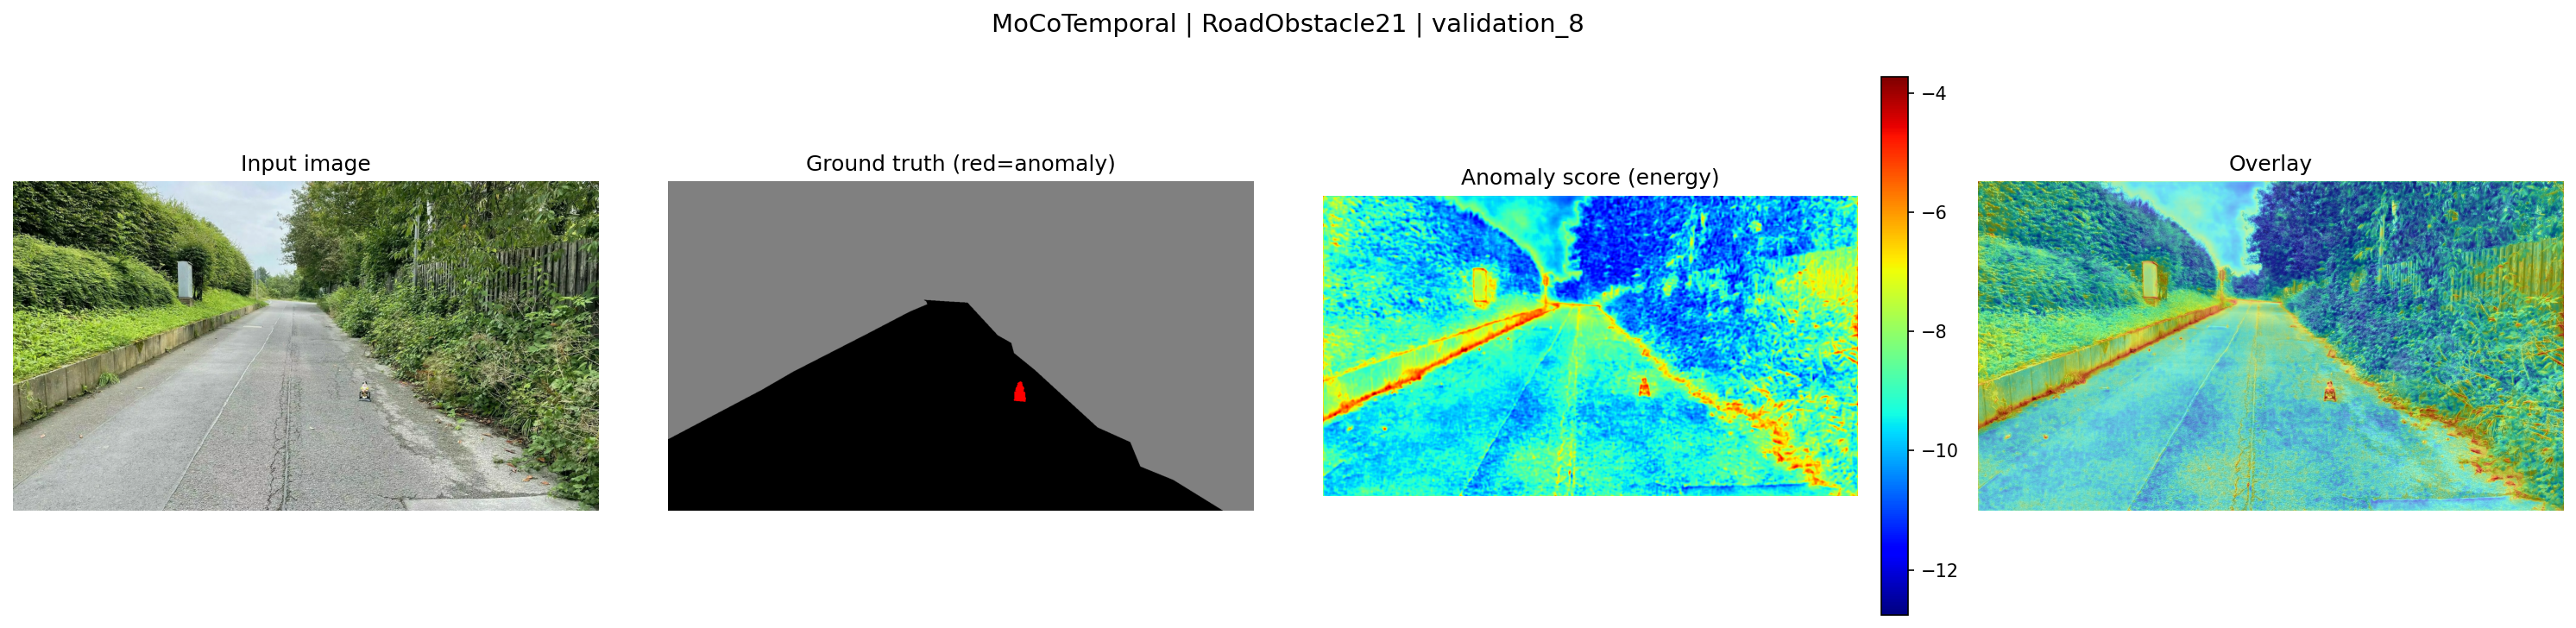
\includegraphics[width=\textwidth]{Figures/kvalitativno/MoCoTemporal_RoadObstacle21_validation_8_energy.png}
	\caption{MoCo temporal model na primjerima iz RoadObstacle21
		validacijskog skupa: crveni kišobran na cesti (gore) i
		mali pas na asfaltu (dolje). Model uspješno lokalizira
		oba objekta, no u donjem primjeru vidljivi su visoki
		anomalni rezultati duž rubova ceste što uzrokuje lažno
		pozitivne detekcije.}
	\label{fig:qual_obstacle}
\end{figure}

\begin{figure}[H]
	\centering
	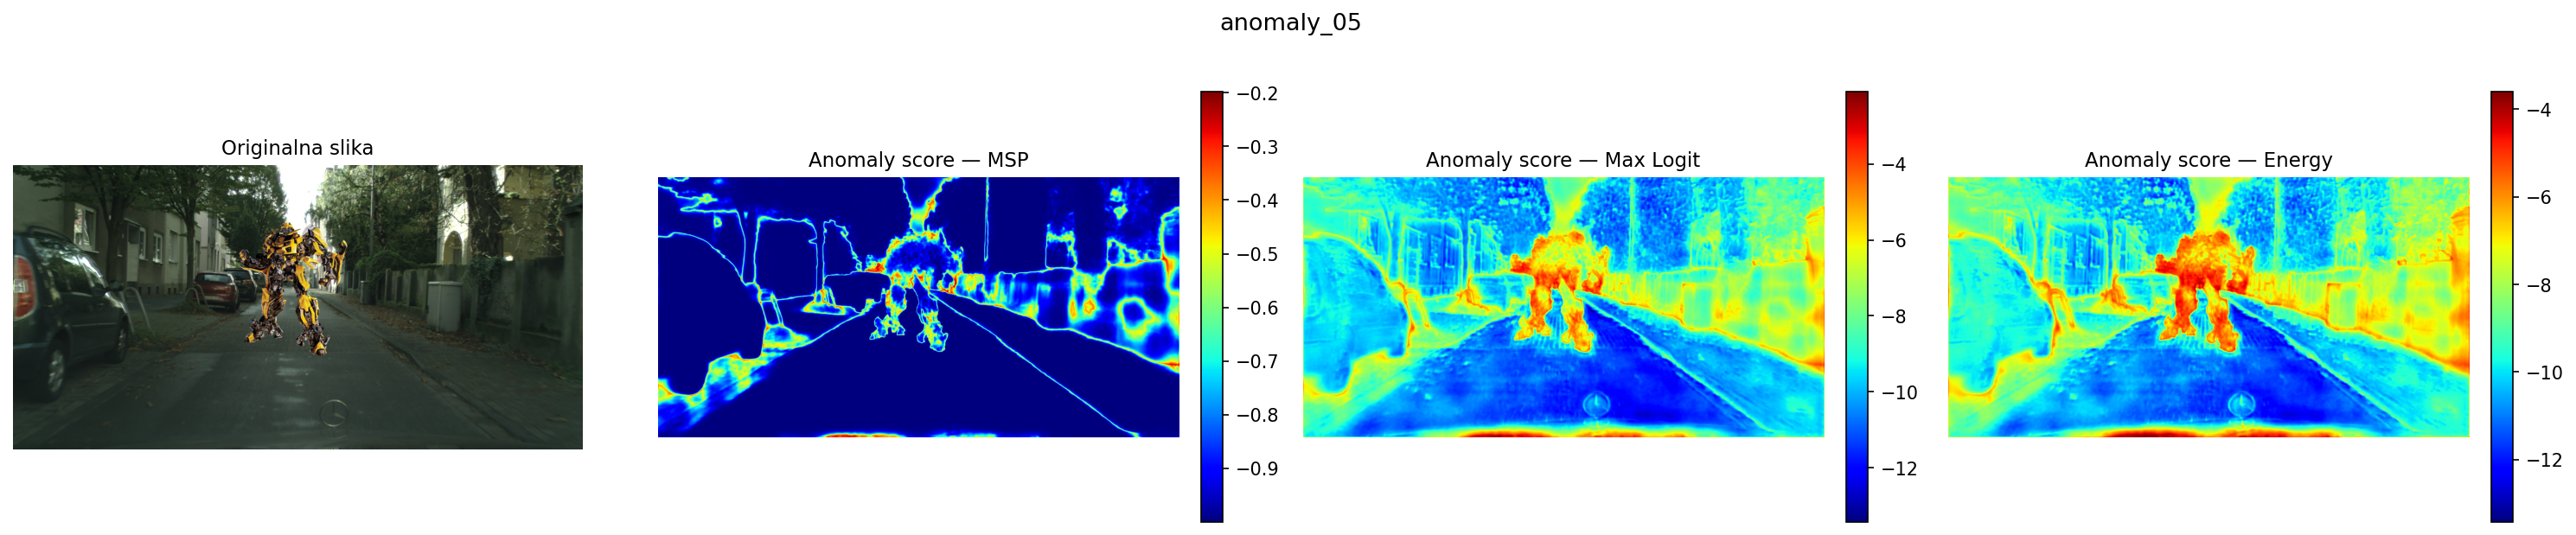
\includegraphics[width=\textwidth]{Figures/kvalitativno/anomaly_05_scores.png}
	\vspace{2mm}
	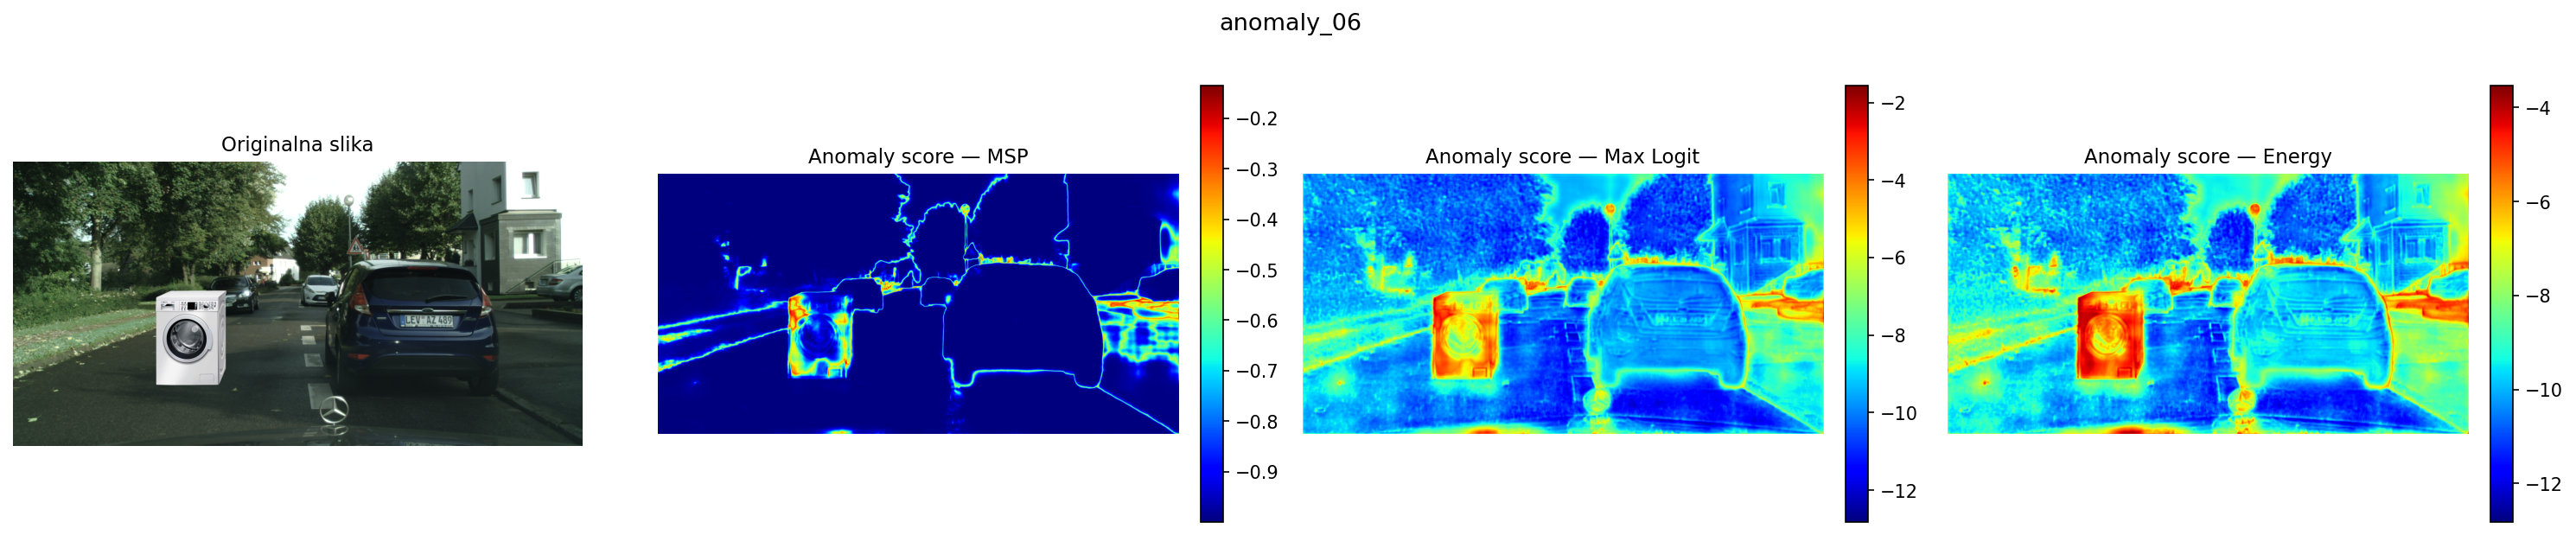
\includegraphics[width=\textwidth]{Figures/kvalitativno/anomaly_06_scores.png}
	\caption{Usporedba triju funkcija ocjenjivanja anomalija (MSP,
		MaxLogit, Energy) na Cityscapes scenama s digitalno
		ubačenim anomalijama: robot (gore) i perilica rublja
		(dolje). MSP funkcija daje znatno niže apsolutne
		vrijednosti i lošiju prostornu lokalizaciju anomalije
		u usporedbi s MaxLogit i Energy funkcijama. Energy i
		MaxLogit pokazuju usporedive rezultate s jasno
		izdvojenim anomalnim objektima.}
	\label{fig:qual_scoring}
\end{figure}

Kvalitativni rezultati otkrivaju nekoliko važnih opažanja. Svi
ispitani modeli uspješno detektiraju velika anomalna tijela poput
helikoptera i traktora koji zauzimaju značajan udio slike. Međutim,
modeli imaju poteškoća s malim anomalijama, primjer psa na cesti
(slika~\ref{fig:qual_obstacle}, dolje) pokazuje da model lokalizira
objekt, ali uz visok anomalni rezultat na rubovima ceste koji
uzrokuju lažno pozitivne detekcije.

Usporedba scoring funkcija (slika~\ref{fig:qual_scoring}) vizualno
potvrđuje numeričke rezultate: MSP funkcija komprimira anomalne
rezultate u uski raspon vrijednosti i ne razlikuje dobro anomalne
od normalnih piksela, dok MaxLogit i Energy daju jasno izdvojeni
signal na anomalnom objektu uz niži šum na pozadini. Energy funkcija
postiže nešto bolju prostornu konzistentnost od MaxLogita, što
odgovara njezinom teorijskom temelju u energetskim modelima.

Zanimljivo je da rubovi i granice objekata sustavno pokazuju više
anomalne rezultate od unutrašnjosti objekata. Ovaj efekt posljedica
je nesigurnosti modela na granicama semantičkih regija, gdje piksel
može biti klasificiran u dvije ili više klasa. U kontekstu detekcije
anomalija to znači da model može "zaokružiti" anomalni objekt i s
unutarnje i s vanjske strane granice, što doprinosi lažno pozitivnim
pikselima.



%--- ZAKLJUČAK / CONCLUSION ----------------------------------------------------
\chapter{Zaključak}
\label{pog:zakljucak}

U ovom radu istražili smo može li samonadzirani predtrening metodom MoCo v2 na neoznačenim video sekvencama prometnih scena poboljšati detekciju anomalija u semantičkoj segmentaciji. Ispitali smo tri varijante: osnovni model s ImageNet inicijalizacijom, MoCo standard s augmentacijama iste slike i MoCo temporal sa susjednim okvirima kao pozitivnim parovima. Rezultati su mješoviti. MoCo standard zaostaje za osnovnim modelom na svim skupovima, dok MoCo temporal blago nadmašuje osnovni model na skupu RoadObstacle21 u AUPRC (7,34\% nasuprot 6,85\%) i značajno u komponentnim metrikama sIoU (18,77\% nasuprot 8,79\%). Na skupu RoadAnomaly21 pak ostaje najuspješniji osnovni model, što je vjerojatno posljedica toga da su tamošnje anomalije vizualno raznolike slike s interneta koje su daleko od prometne domene na kojoj smo provodili predtrening. Zaključno, ne možemo tvrditi da samonadzirani predtrening konzistentno pomaže, ali možemo reći da temporalni signal daje bolji nadzorni signal od augmentacija iste slike. Uz duži predtrening, veće skupove podataka i novije SSL metode poput DINO-a, rezultati bi vjerojatno bili bolji.

%--- LITERATURA / REFERENCES ---------------------------------------------------

% Literatura se automatski generira iz zadane .bib datoteke / References are automatically generated from the supplied .bib file
% Upiši ime BibTeX datoteke bez .bib nastavka / Enter the name of the BibTeX file without .bib extension
\bibliography{literatura}



%--- SAŽETAK / ABSTRACT --------------------------------------------------------

% Sažetak na hrvatskom
\begin{sazetak}
	Ovaj rad istražuje primjenu samonadziranog učenja za poboljšanje detekcije anomalija u prometnim scenama. Predloženi sustav sastoji se od triju faza: samonadziranog predtreninga okosnice ResNet50 metodom MoCo v2 na neoznačenim okvirima skupa Cityscapes-Sequence, segmentacijskog dotreniranja modela DeepLabV3+ na označenom Cityscapes skupu te post-hoc detekcije anomalija funkcijama Maximum Softmax Probability, Maximum Logit i Energy. Ispituju se dvije varijante predtreninga: standardna s augmentacijama iste slike kao pozitivnim parovima, i temporalna sa susjednim okvirima iste video sekvence. Evaluacija se provodi na SegmentMeIfYouCan benchmarku. Rezultati pokazuju da temporalna varijanta konzistentno nadmašuje standardnu na svim skupovima. Međutim, samonadzirani predtrening nije konzistentno poboljšao detekciju u odnosu na osnovni model. Na skupu RoadObstacle21 MoCo temporal postiže sIoU od 18,77\% nasuprot 8,79\% osnovnog modela.
\end{sazetak}

\begin{kljucnerijeci}
	detekcija anomalija; samonadzirano učenje; kontrastivno učenje; semantička segmentacija; prometne scene; MoCo v2; temporalno kontrastivno učenje; izvandistribucijska detekcija
\end{kljucnerijeci}


% Abstract in English
\begin{abstract}
	The thesis investigates the application of self-supervised learning for improving anomaly detection in traffic scenes. The proposed system consists of three phases: self-supervised pretraining of a ResNet50 backbone using MoCo v2 on unlabeled frames from the Cityscapes-Sequence dataset, supervised fine-tuning of a DeepLabV3+ model on the annotated Cityscapes dataset, and post-hoc anomaly detection using Maximum Softmax Probability, Maximum Logit, and Energy scoring functions. Two pretraining variants are evaluated: a standard variant using augmentations of the same image as positive pairs, and a temporal variant using adjacent frames from the same video sequence. Evaluation is conducted on the SegmentMeIfYouCan benchmark. Results show that the temporal variant consistently outperforms the standard variant across all evaluated datasets. However, self-supervised pretraining did not consistently improve anomaly detection compared to the baseline model. On the RoadObstacle21 subset, MoCo temporal achieves an sIoU of 18.77\% compared to 8.79\% for the baseline model.
\end{abstract}

\begin{keywords}
	anomaly detection; self-supervised learning; contrastive learning; semantic segmentation; traffic scenes; MoCo v2; temporal contrastive learning; out-of-distribution detection
\end{keywords}


%--- PRIVITCI / APPENDIX -------------------------------------------------------

% Sva poglavlja koja slijede će biti označena slovom i riječi privitak / All following chapters will be denoted with an appendix and a letter
\backmatter

\chapter{Programski kod}

Cjelokupni programski kod razvijen u sklopu ovog rada javno je dostupan na platformi GitHub:

\begin{itemize}
	\item \textbf{Implementacija sustava} (modeli, treniranje, evaluacija): \\
	\url{https://github.com/doms911/traffic-anomaly-ssl}
	
	\item \textbf{Izvorni kod diplomskog rada} (LaTeX): \\
	\url{https://github.com/doms911/master-thesis-traffic-anomaly-ssl}
\end{itemize}

Repozitorij implementacije sadrži sve komponente sustava: definicije modela (MoCo v2, DeepLabV3+), skripte za samonadzirani predtrening i segmentacijsko dotreniranje, evaluacijski pipeline za SMIYC benchmark te skripte za generiranje vizualizacija korištenih u radu.


\end{document}
